\appendix
\section*{Appendix}
\addcontentsline{toc}{section}{Appendix}

\subsection*{Code and Supplementary Materials}

This project and its components are stored in an open-access GitHub repository that documents the full research process—from early exploration and background preparation to final analysis, figures, and written materials. The repository is structured to showcase the broader development of the project, including legacy scripts, processed outputs, and dissertation documentation.

\vspace{1em}
\subsubsection*{Repository Overview}

\begin{itemize}
  \item \textbf{code} – Core Python scripts used in the analysis, grouped by stage: \textbf{data\_processing}, \textbf{journey\_builder}, and \textbf{metrics}. A \textbf{utils} folder contains shared helper functions.

  \item \textbf{data} – Outputs of the analysis, including processed metrics and spatial reference files. The raw AVLS forecast data is excluded due to file size limitations.

  \item \textbf{figures} – All visualisations produced during the analysis, grouped by pandemic phase and performance metric. Appendix figures are included.

  \item \textbf{archive} – Background materials, legacy scripts, and early data outputs.

  \item \textbf{documentation} – LaTeX source files for the dissertation, including bibliography, formatting settings, and style files.

  \item \textbf{README.md} – Setup instructions, environment details, and an overview of repository logic.
\end{itemize}

\vspace{1em}
\subsubsection*{GitHub Repository}

The repository is available at:

\url{https://github.com/rodriguesathena/TCD_Dissertation}

Note: Due to file size limitations, raw AVLS forecast data is not included. However, it is publicly accessible via the original archive (as cited in the bibliography). All processing scripts and figure-generation code are included for full transparency and replication.

% --------------------------------------------------
\newpage
\subsection*{Headway Regularity}

\subsubsection*{Headway Percentage}
\begin{table}[H]
  \centering
  \caption{Percentage of stops with average peak-period Headways exceeding 10 minutes}
  \label{tab:headway_summary}
  \begin{tabular}{lcc}
    \textbf{Period} & \textbf{Green Line (\%)} & \textbf{Red Line (\%)} \\
    Pre-COVID & 63.7 & 75.2 \\
    Lockdown  & 62.1 & 71.8 \\
    Recovery  & 79.8 & 81.8 \\
    Post-COVID & 85.5 & 96.4 \\
  \end{tabular}
\end{table}

\subsubsection*{Average Peak Period Headways}

\begin{figure}[H]
  \centering
  \includegraphics[width=0.49\textwidth]{figures/appendix_figures/headway_regularity/headways_combined_green_precovid.png}
  \includegraphics[width=0.49\textwidth]{figures/appendix_figures/headway_regularity/headways_combined_red_precovid.png}
  \caption{Pre-COVID}
\end{figure}

\begin{figure}[H]
  \centering
  \includegraphics[width=0.49\textwidth]{figures/appendix_figures/headway_regularity/headways_combined_green_lockdown.png}
  \includegraphics[width=0.49\textwidth]{figures/appendix_figures/headway_regularity/headways_combined_red_lockdown.png}
  \caption{Lockdown}
\end{figure}

\begin{figure}[H]
  \centering
  \includegraphics[width=0.49\textwidth]{figures/appendix_figures/headway_regularity/headways_combined_green_recovery.png}
  \includegraphics[width=0.49\textwidth]{figures/appendix_figures/headway_regularity/headways_combined_red_recovery.png}
  \caption{Recovery}
\end{figure}

\begin{figure}[H]
  \centering
  \includegraphics[width=0.49\textwidth]{figures/appendix_figures/headway_regularity/headways_combined_green_postcovid.png}
  \includegraphics[width=0.49\textwidth]{figures/appendix_figures/headway_regularity/headways_combined_red_postcovid.png}
  \caption{Post-COVID}
\end{figure}

% --------------------------------------------------
\newpage
\subsection*{Travel Time Volatility}

\subsubsection*{Volatility Below the Threshold}
\begin{table}[H]
  \centering
  \caption{Percentage of stop-pairs with travel time volatility (TTV) below 1 minute}
  \label{tab:ttv_summary}
  \begin{tabular}{lcc}
    \textbf{Phase} & \textbf{\% Below 1 Min} & \textbf{Max Volatility (min)} \\
    Pre-COVID & 77.66 & 4.28 \\
    Lockdown  & 74.56 & 4.94 \\
    Recovery  & 73.84 & 4.27 \\
    Post-COVID & 72.63 & 4.24 \\
  \end{tabular}
\end{table}

\subsubsection*{Travel Time Volatility Figures}

\begin{figure}[H]
  \centering
  \includegraphics[width=0.85\textwidth]{figures/appendix_figures/travel_time_volatility/volatility_allperiods_green_combined_precovid.png}
  \includegraphics[width=0.85\textwidth]{figures/appendix_figures/travel_time_volatility/volatility_allperiods_red_combined_precovid.png}
  \caption{Pre-COVID}
\end{figure}

\vspace{5cm}
\begin{figure}[H]
  \centering
  \includegraphics[width=0.85\textwidth]{figures/appendix_figures/travel_time_volatility/volatility_allperiods_green_combined_lockdown.png}
  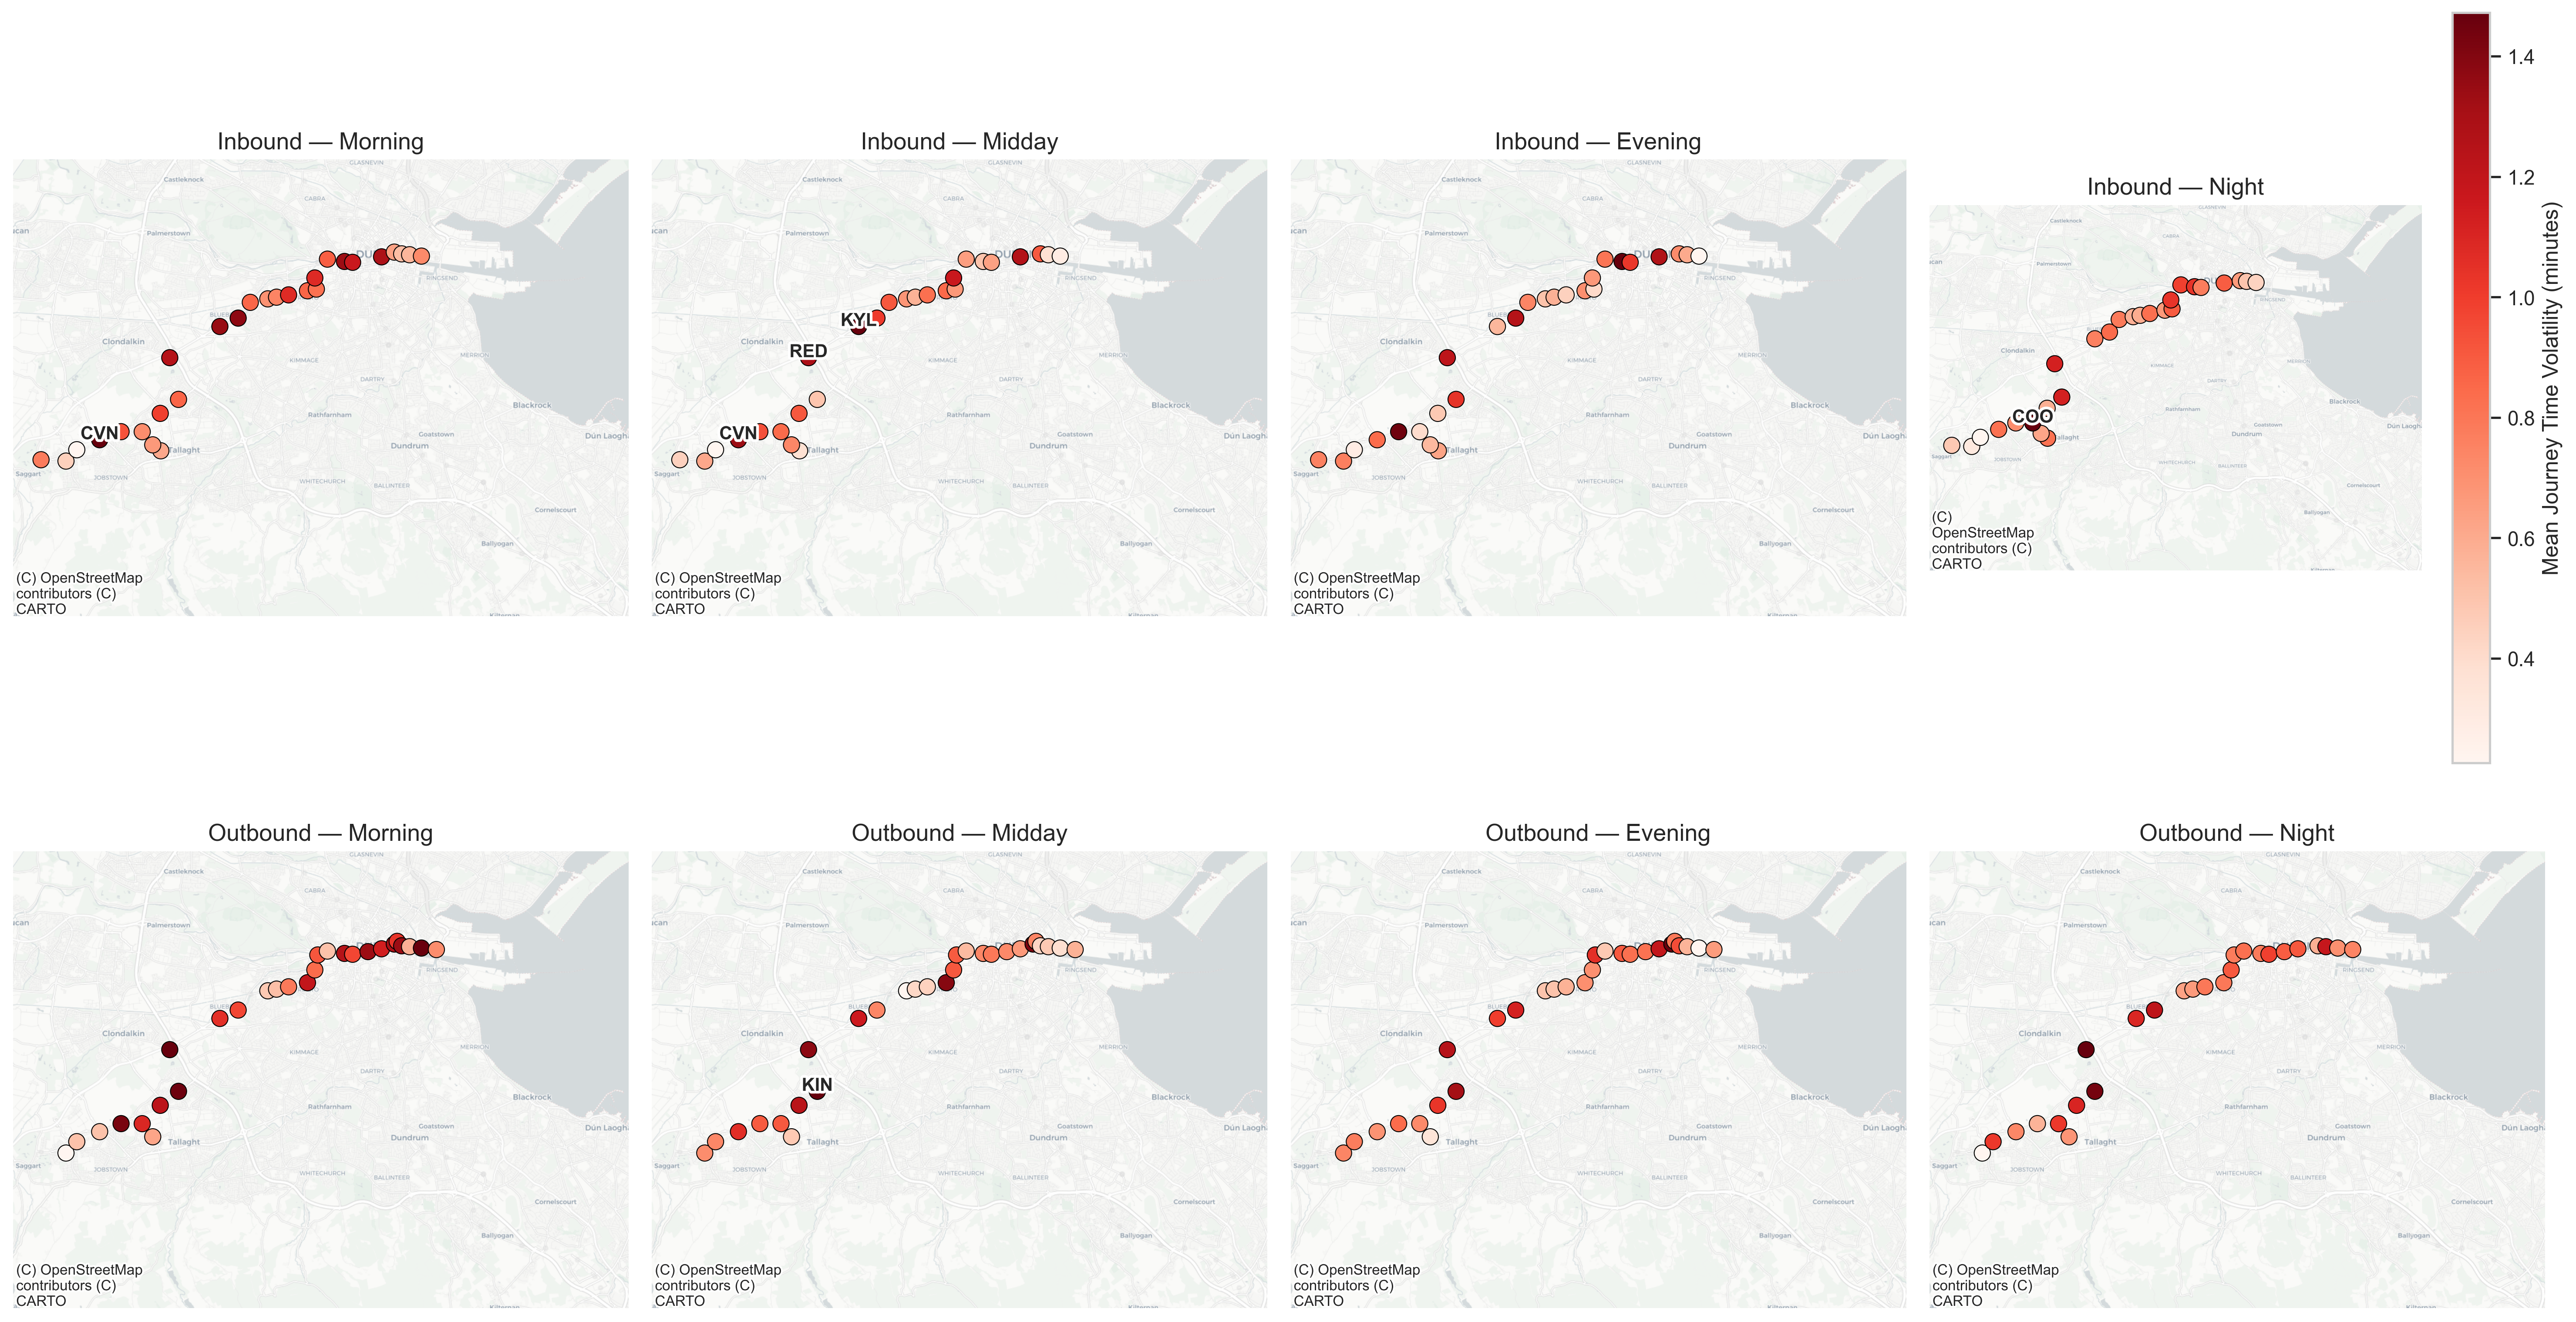
\includegraphics[width=0.85\textwidth]{figures/appendix_figures/travel_time_volatility/volatility_allperiods_red_combined_lockdown.png}
  \caption{Lockdown}
\end{figure}

\vspace{5cm}

\begin{figure}[H]
  \centering
  \includegraphics[width=0.85\textwidth]{figures/appendix_figures/travel_time_volatility/volatility_allperiods_green_combined_recovery.png}
  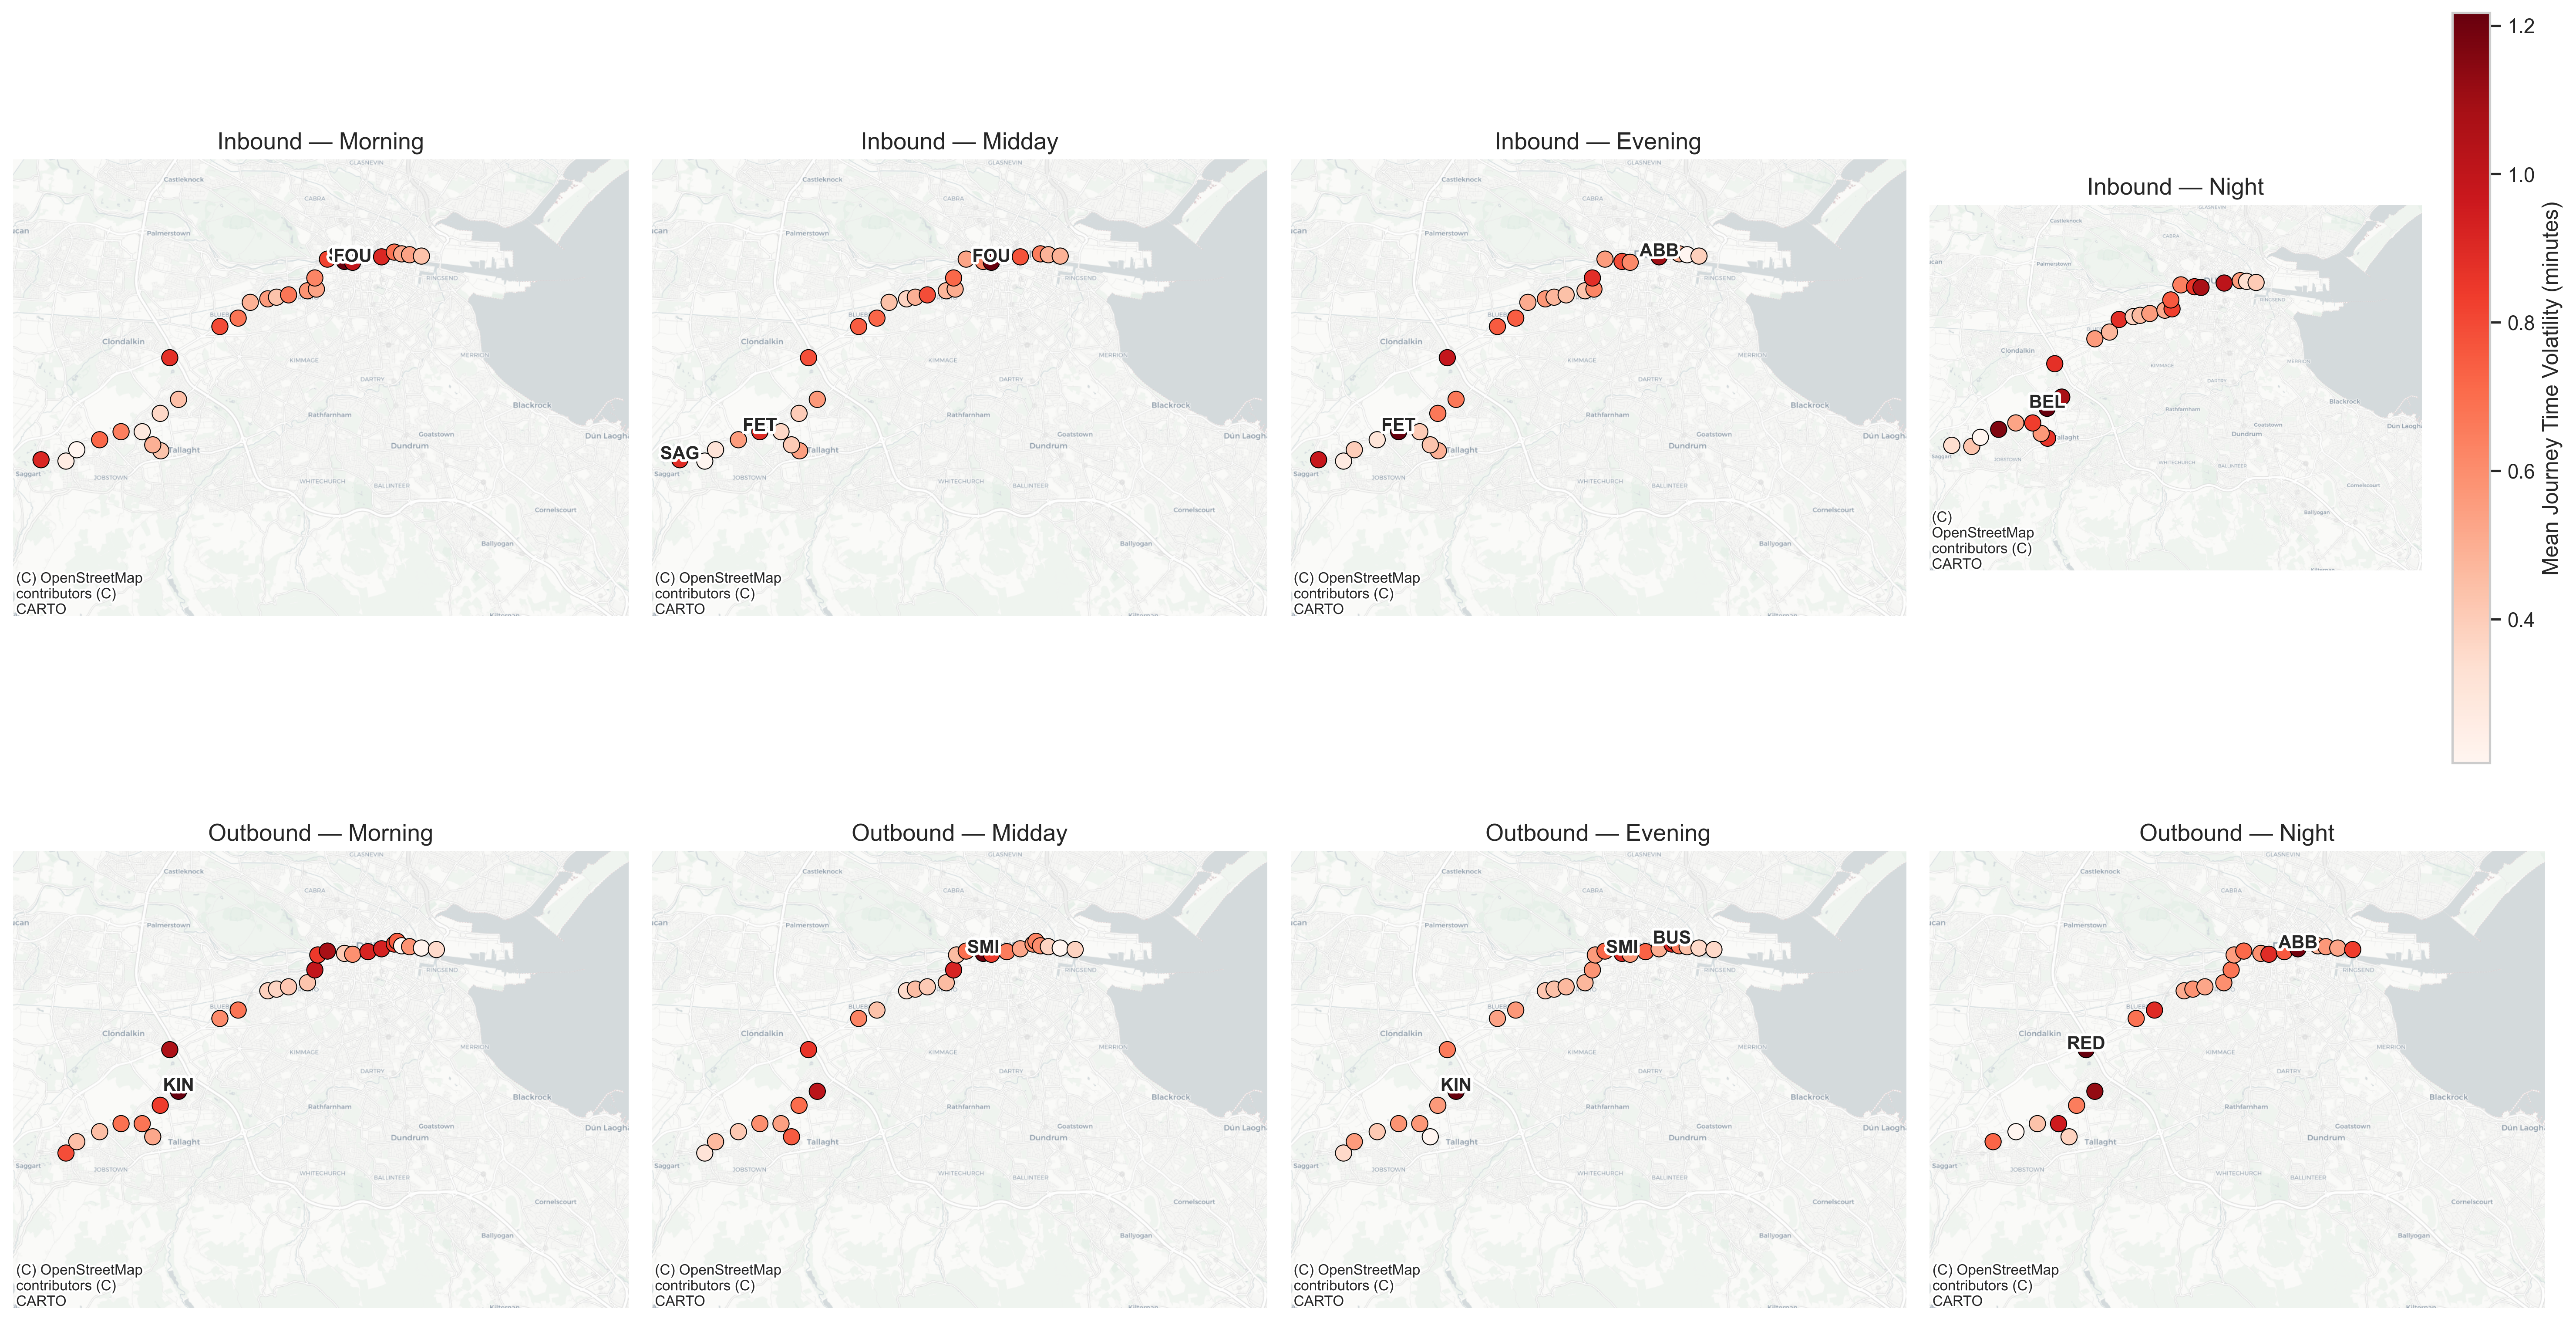
\includegraphics[width=0.85\textwidth]{figures/appendix_figures/travel_time_volatility/volatility_allperiods_red_combined_recovery.png}
  \caption{Recovery}
\end{figure}

\vspace{5cm}
\begin{figure}[H]
  \centering
  \includegraphics[width=0.85\textwidth]{figures/appendix_figures/travel_time_volatility/volatility_allperiods_green_combined_postcovid.png}
  \includegraphics[width=0.85\textwidth]{figures/appendix_figures/travel_time_volatility/volatility_allperiods_red_combined_postcovid.png}
  \caption{Post-COVID}
\end{figure}

% --------------------------------------------------
\newpage
\subsection*{Journey Duration}

\subsubsection*{Duration Across Varied Groups}

\begin{table}[H]
  \centering
  \caption{Average journey durations by phase and line}
  \label{tab:duration_by_phase}
  \begin{tabular}{lcc}
    \textbf{Period} & \textbf{Green Line (min)} & \textbf{Red Line (min)} \\
    Pre-COVID & 50.2 & 48.5 \\
    Lockdown  & 49.8 & 48.2 \\
    Recovery  & 50.2 & 48.9 \\
    Post-COVID & 50.8 & 49.2 \\
  \end{tabular}
\end{table}

\begin{table}[H]
  \centering
  \caption{Time-of-day journey durations }
  \label{tab:duration_by_time}
  \begin{tabular}{lcccc}
    \textbf{Period} & \textbf{Line} & \textbf{Morning} & \textbf{Evening} & \textbf{Night} \\
    Pre-COVID & Green & 49.7 & 47.8 & 55.8 \\
              & Red   & 48.4 & 49.1 & 47.4 \\
    Lockdown  & Green & 49.6 & 47.4 & 55.2 \\
              & Red   & 48.1 & 48.5 & 47.3 \\
    Recovery  & Green & 49.9 & 48.3 & 55.0 \\
              & Red   & 48.8 & 49.2 & 47.8 \\
    Post-COVID & Green & 50.4 & 48.5 & 56.3 \\
              & Red   & 49.0 & 49.7 & 48.3 \\
  \end{tabular}
\end{table}

\subsubsection*{Journey Duration Figures}

\begin{figure}[H]
  \centering
  \begin{subfigure}[t]{0.49\textwidth}
    \centering
    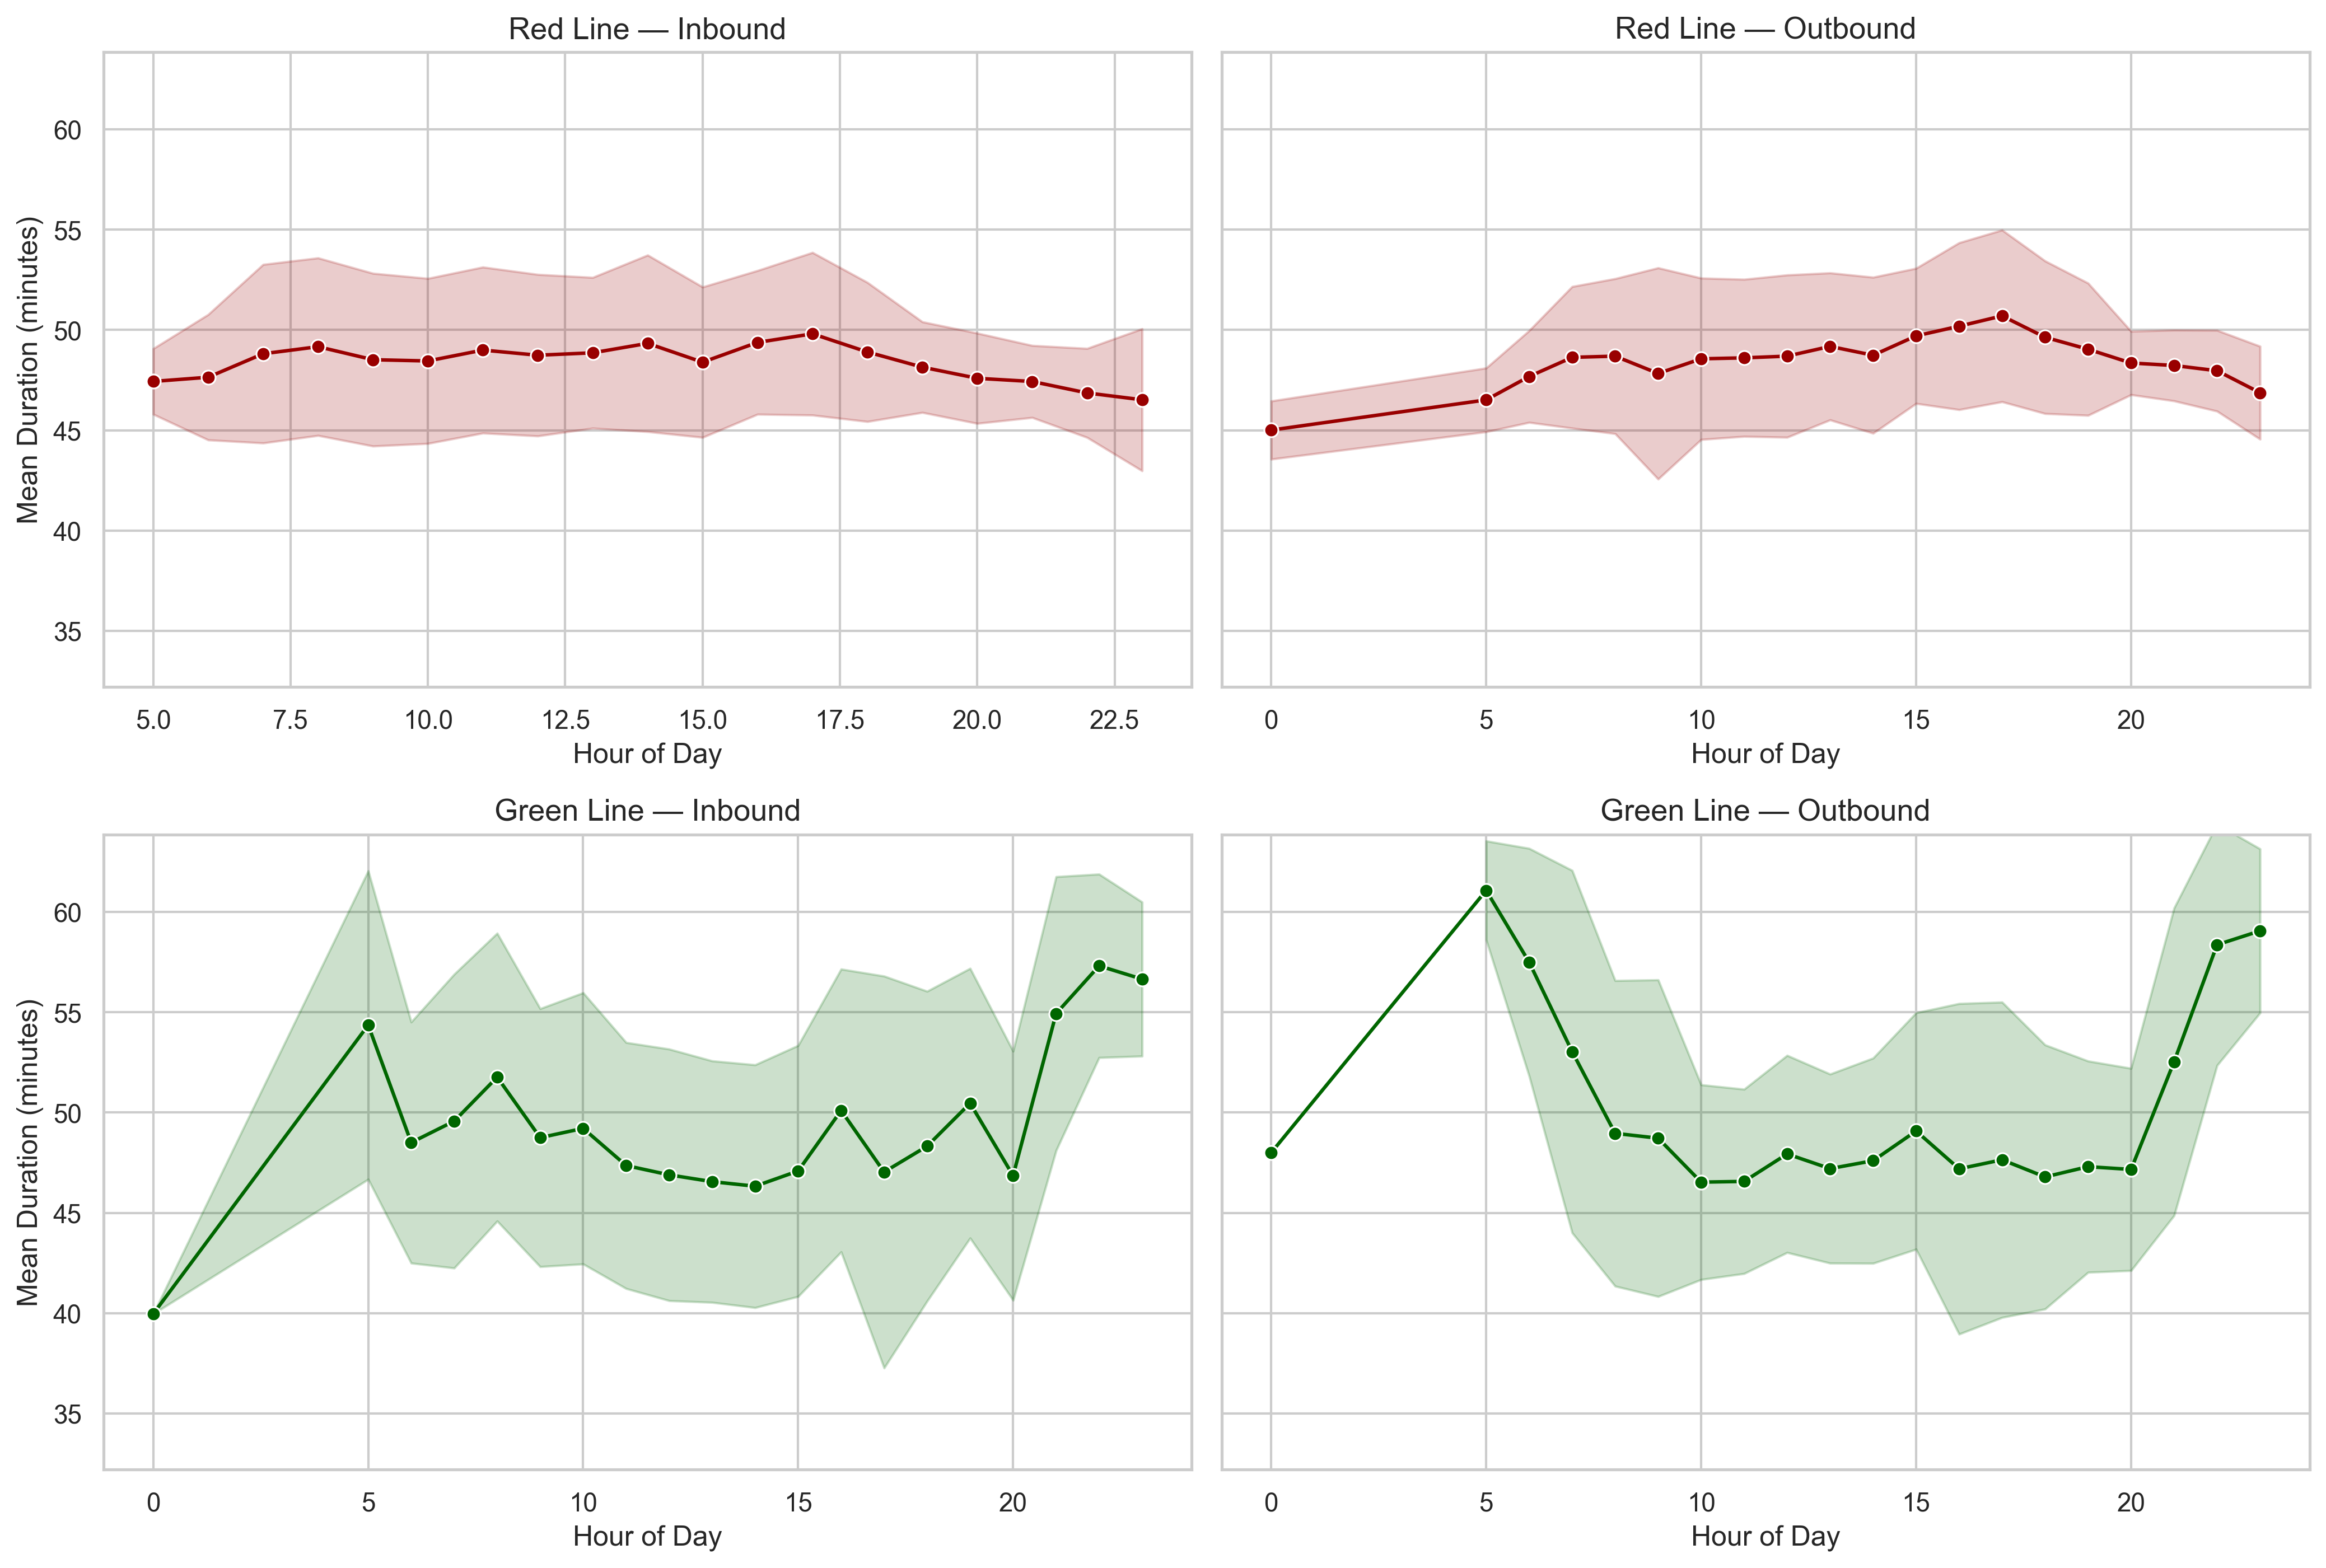
\includegraphics[width=\textwidth]{figures/appendix_figures/journey_duration/duration_hourly_combined_precovid.png}
    \caption*{By Hour}
  \end{subfigure}
  \hfill
  \begin{subfigure}[t]{0.49\textwidth}
    \centering
    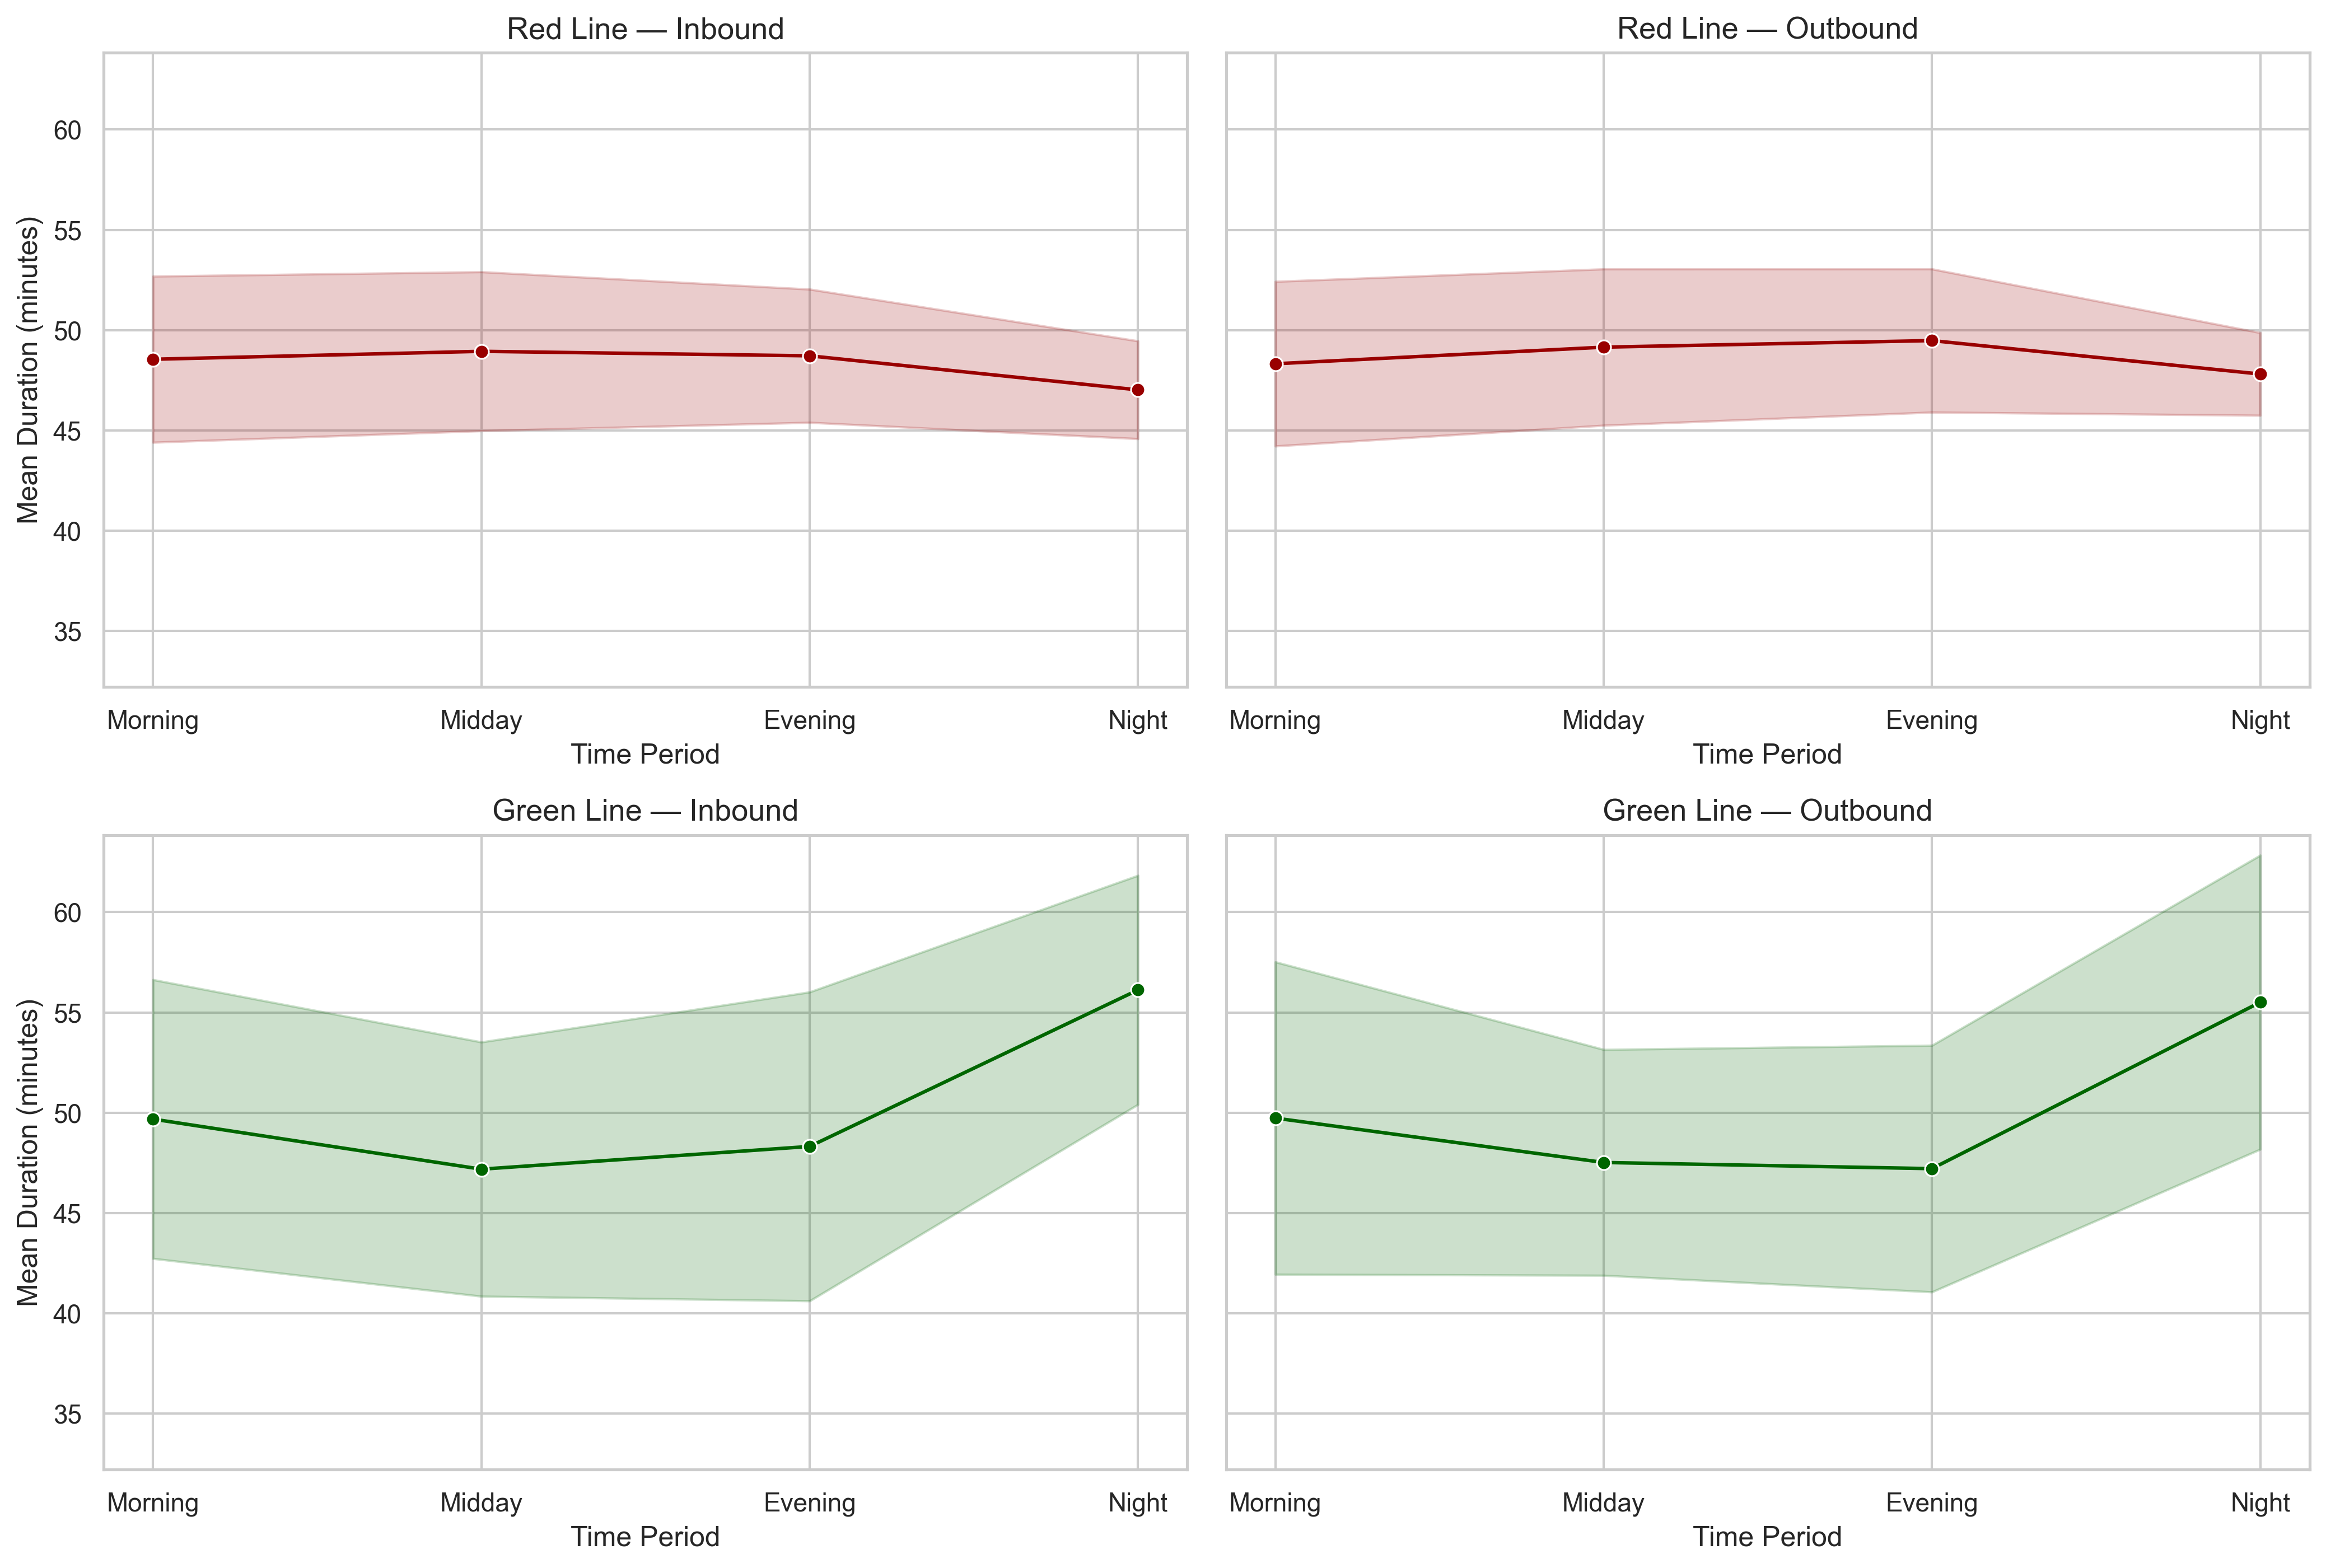
\includegraphics[width=\textwidth]{figures/appendix_figures/journey_duration/duration_period_combined_precovid.png}
    \caption*{By Time-of-Day}
  \end{subfigure}
  \caption{Pre-COVID}
\end{figure}

\begin{figure}[H]
  \centering
  \begin{subfigure}[t]{0.49\textwidth}
    \centering
    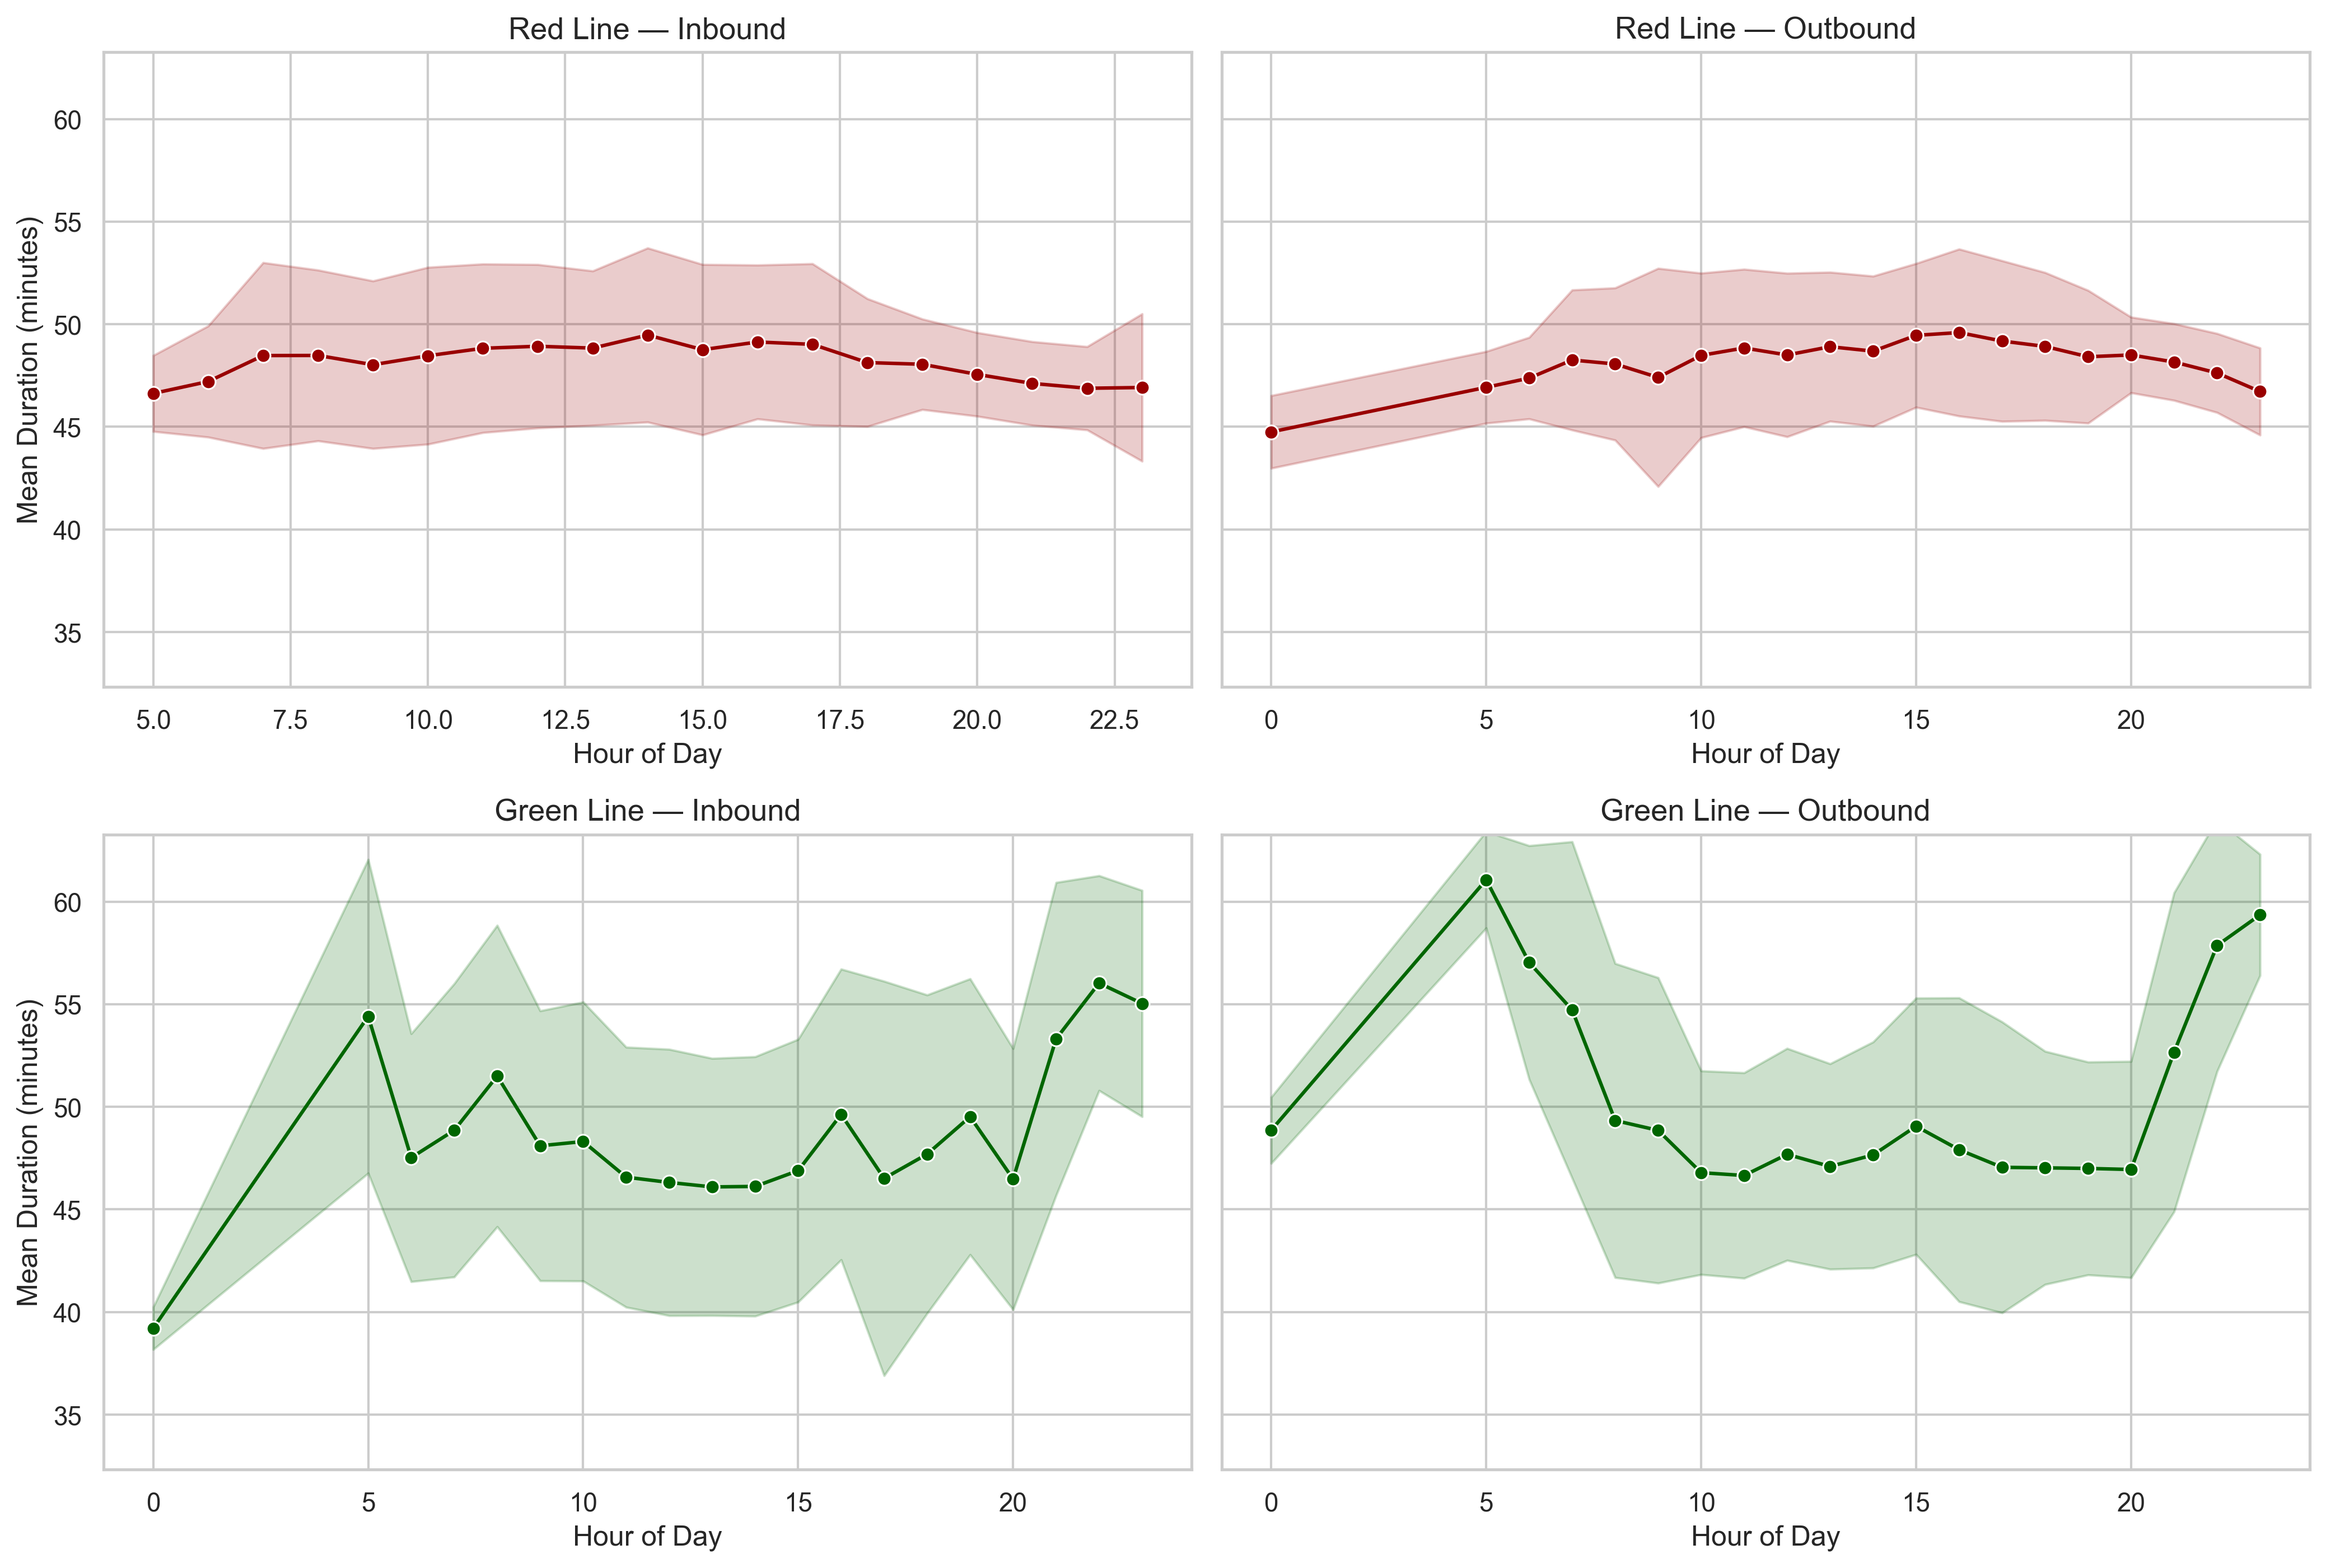
\includegraphics[width=\textwidth]{figures/appendix_figures/journey_duration/duration_hourly_combined_lockdown.png}
    \caption*{By Hour}
  \end{subfigure}
  \hfill
  \begin{subfigure}[t]{0.49\textwidth}
    \centering
    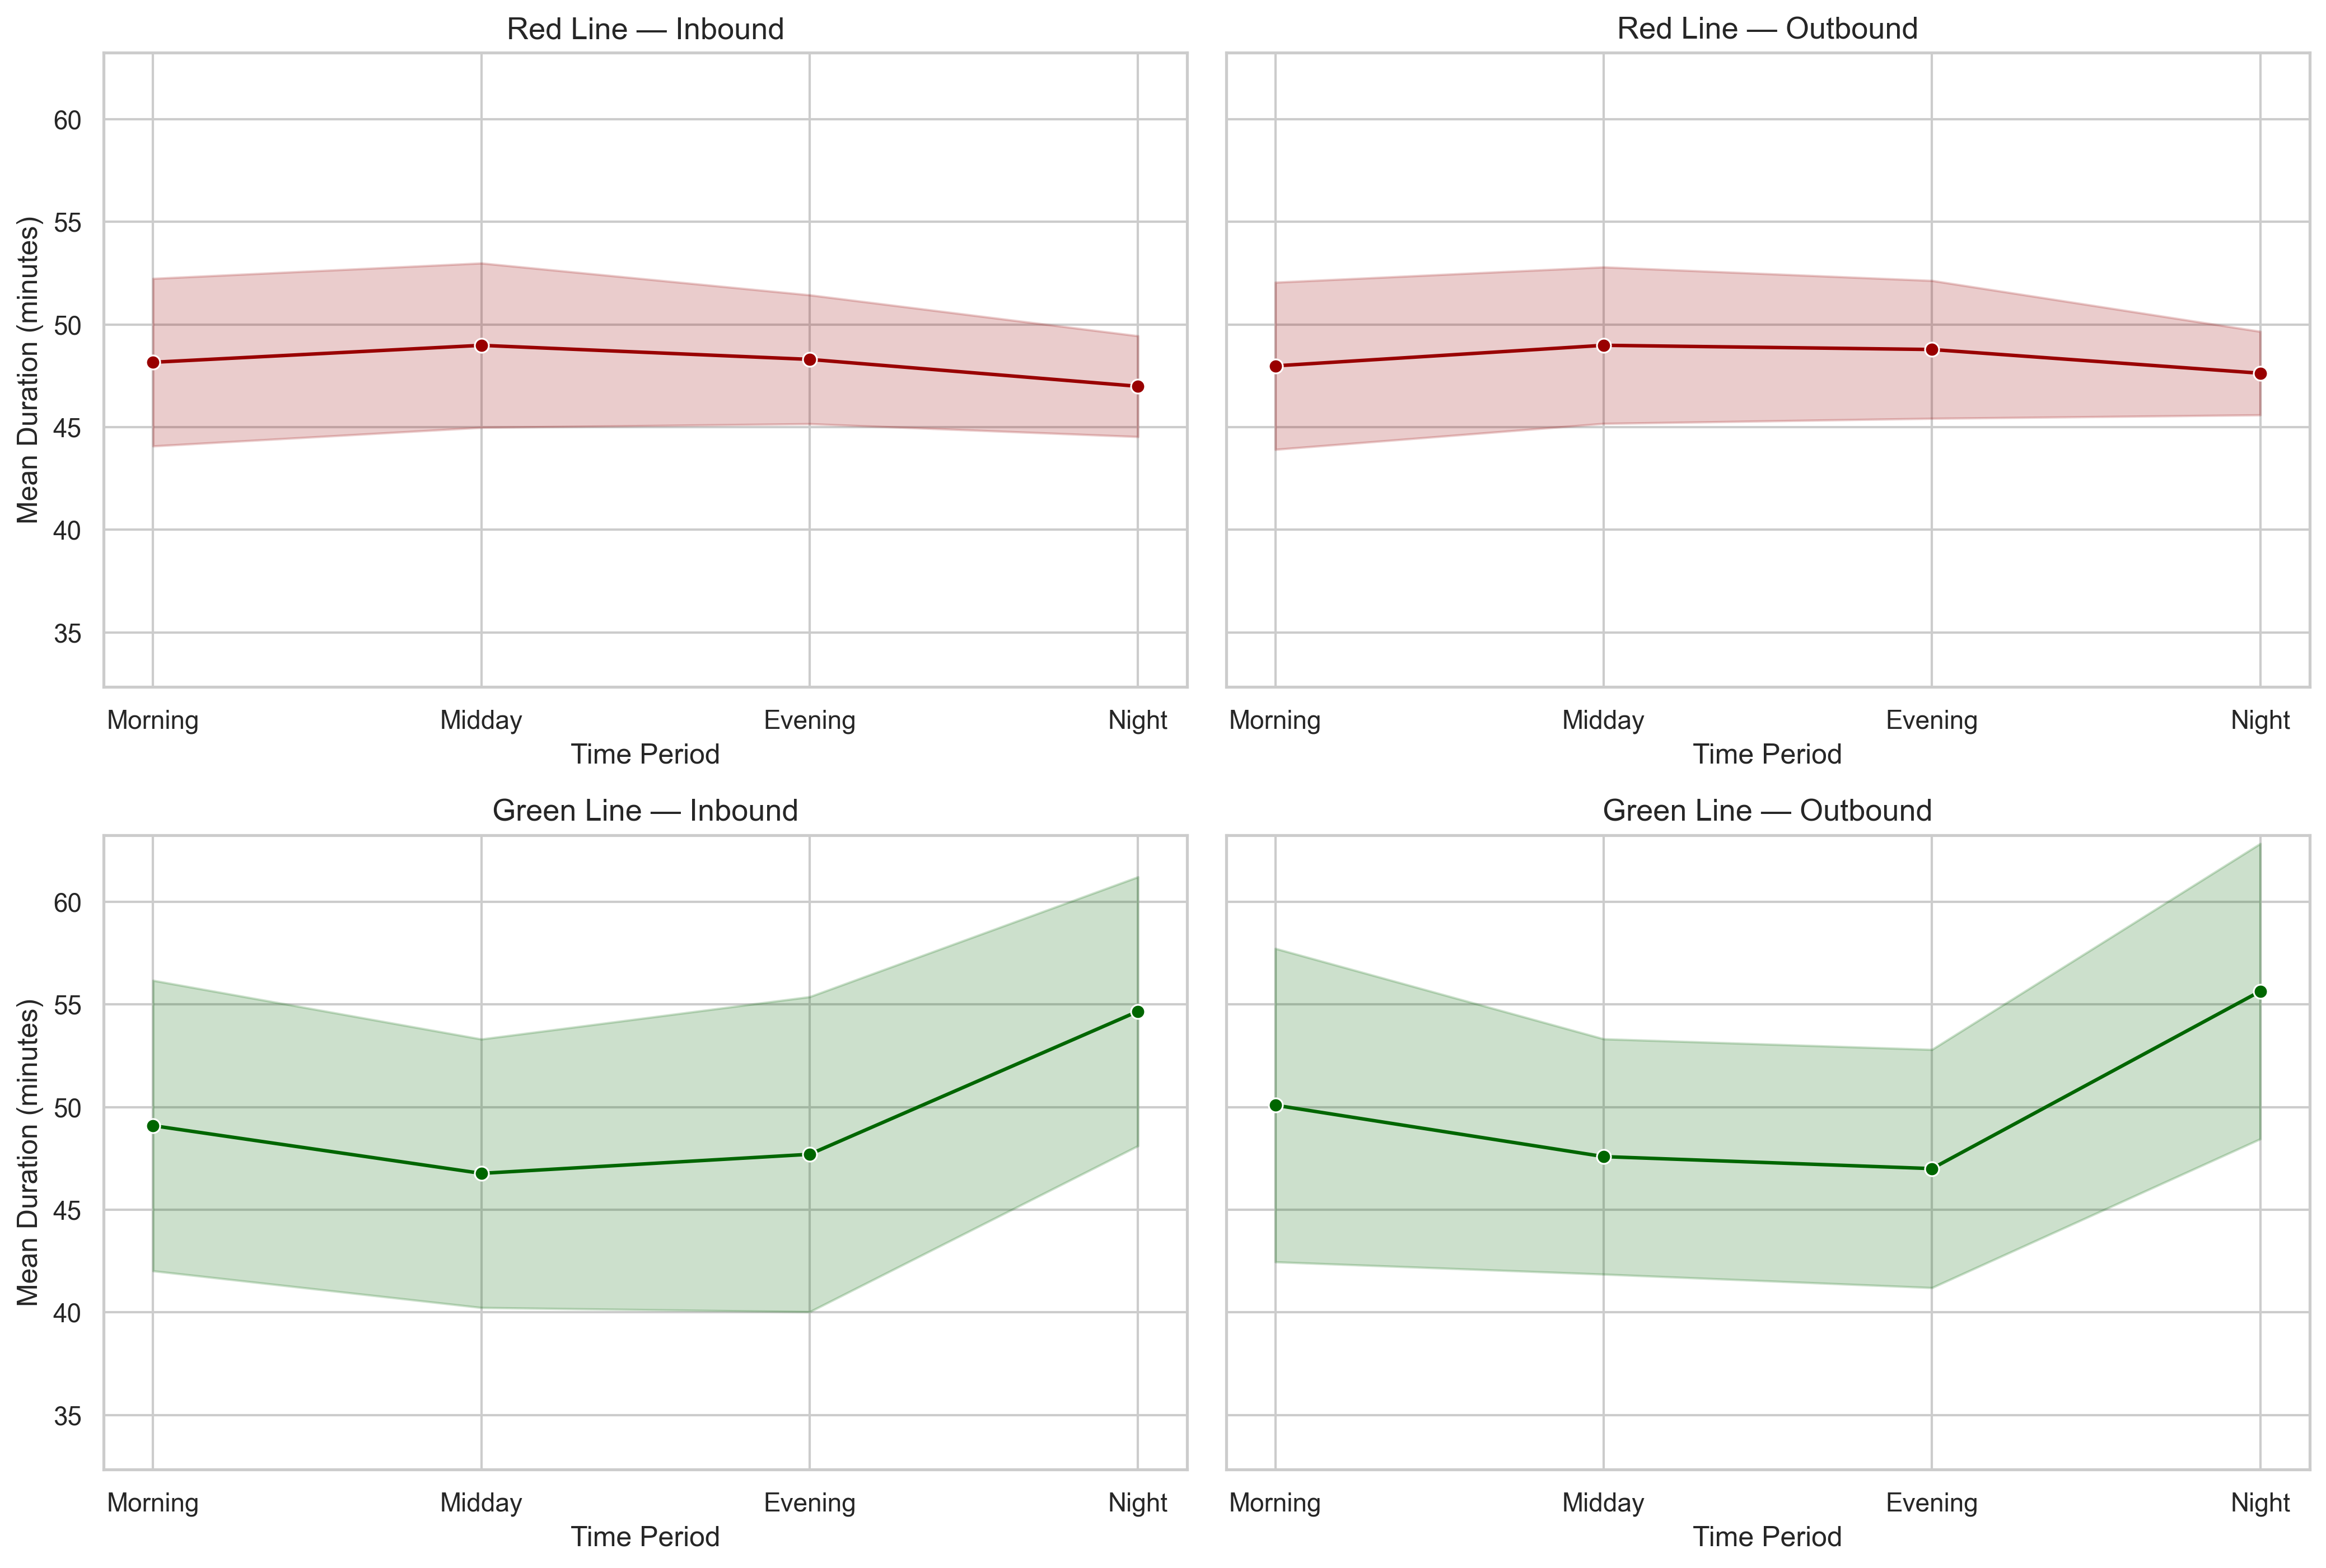
\includegraphics[width=\textwidth]{figures/appendix_figures/journey_duration/duration_period_combined_lockdown.png}
    \caption*{By Time-of-Day}
  \end{subfigure}
  \caption{Lockdown}
\end{figure}

\begin{figure}[H]
  \centering
  \begin{subfigure}[t]{0.49\textwidth}
    \centering
    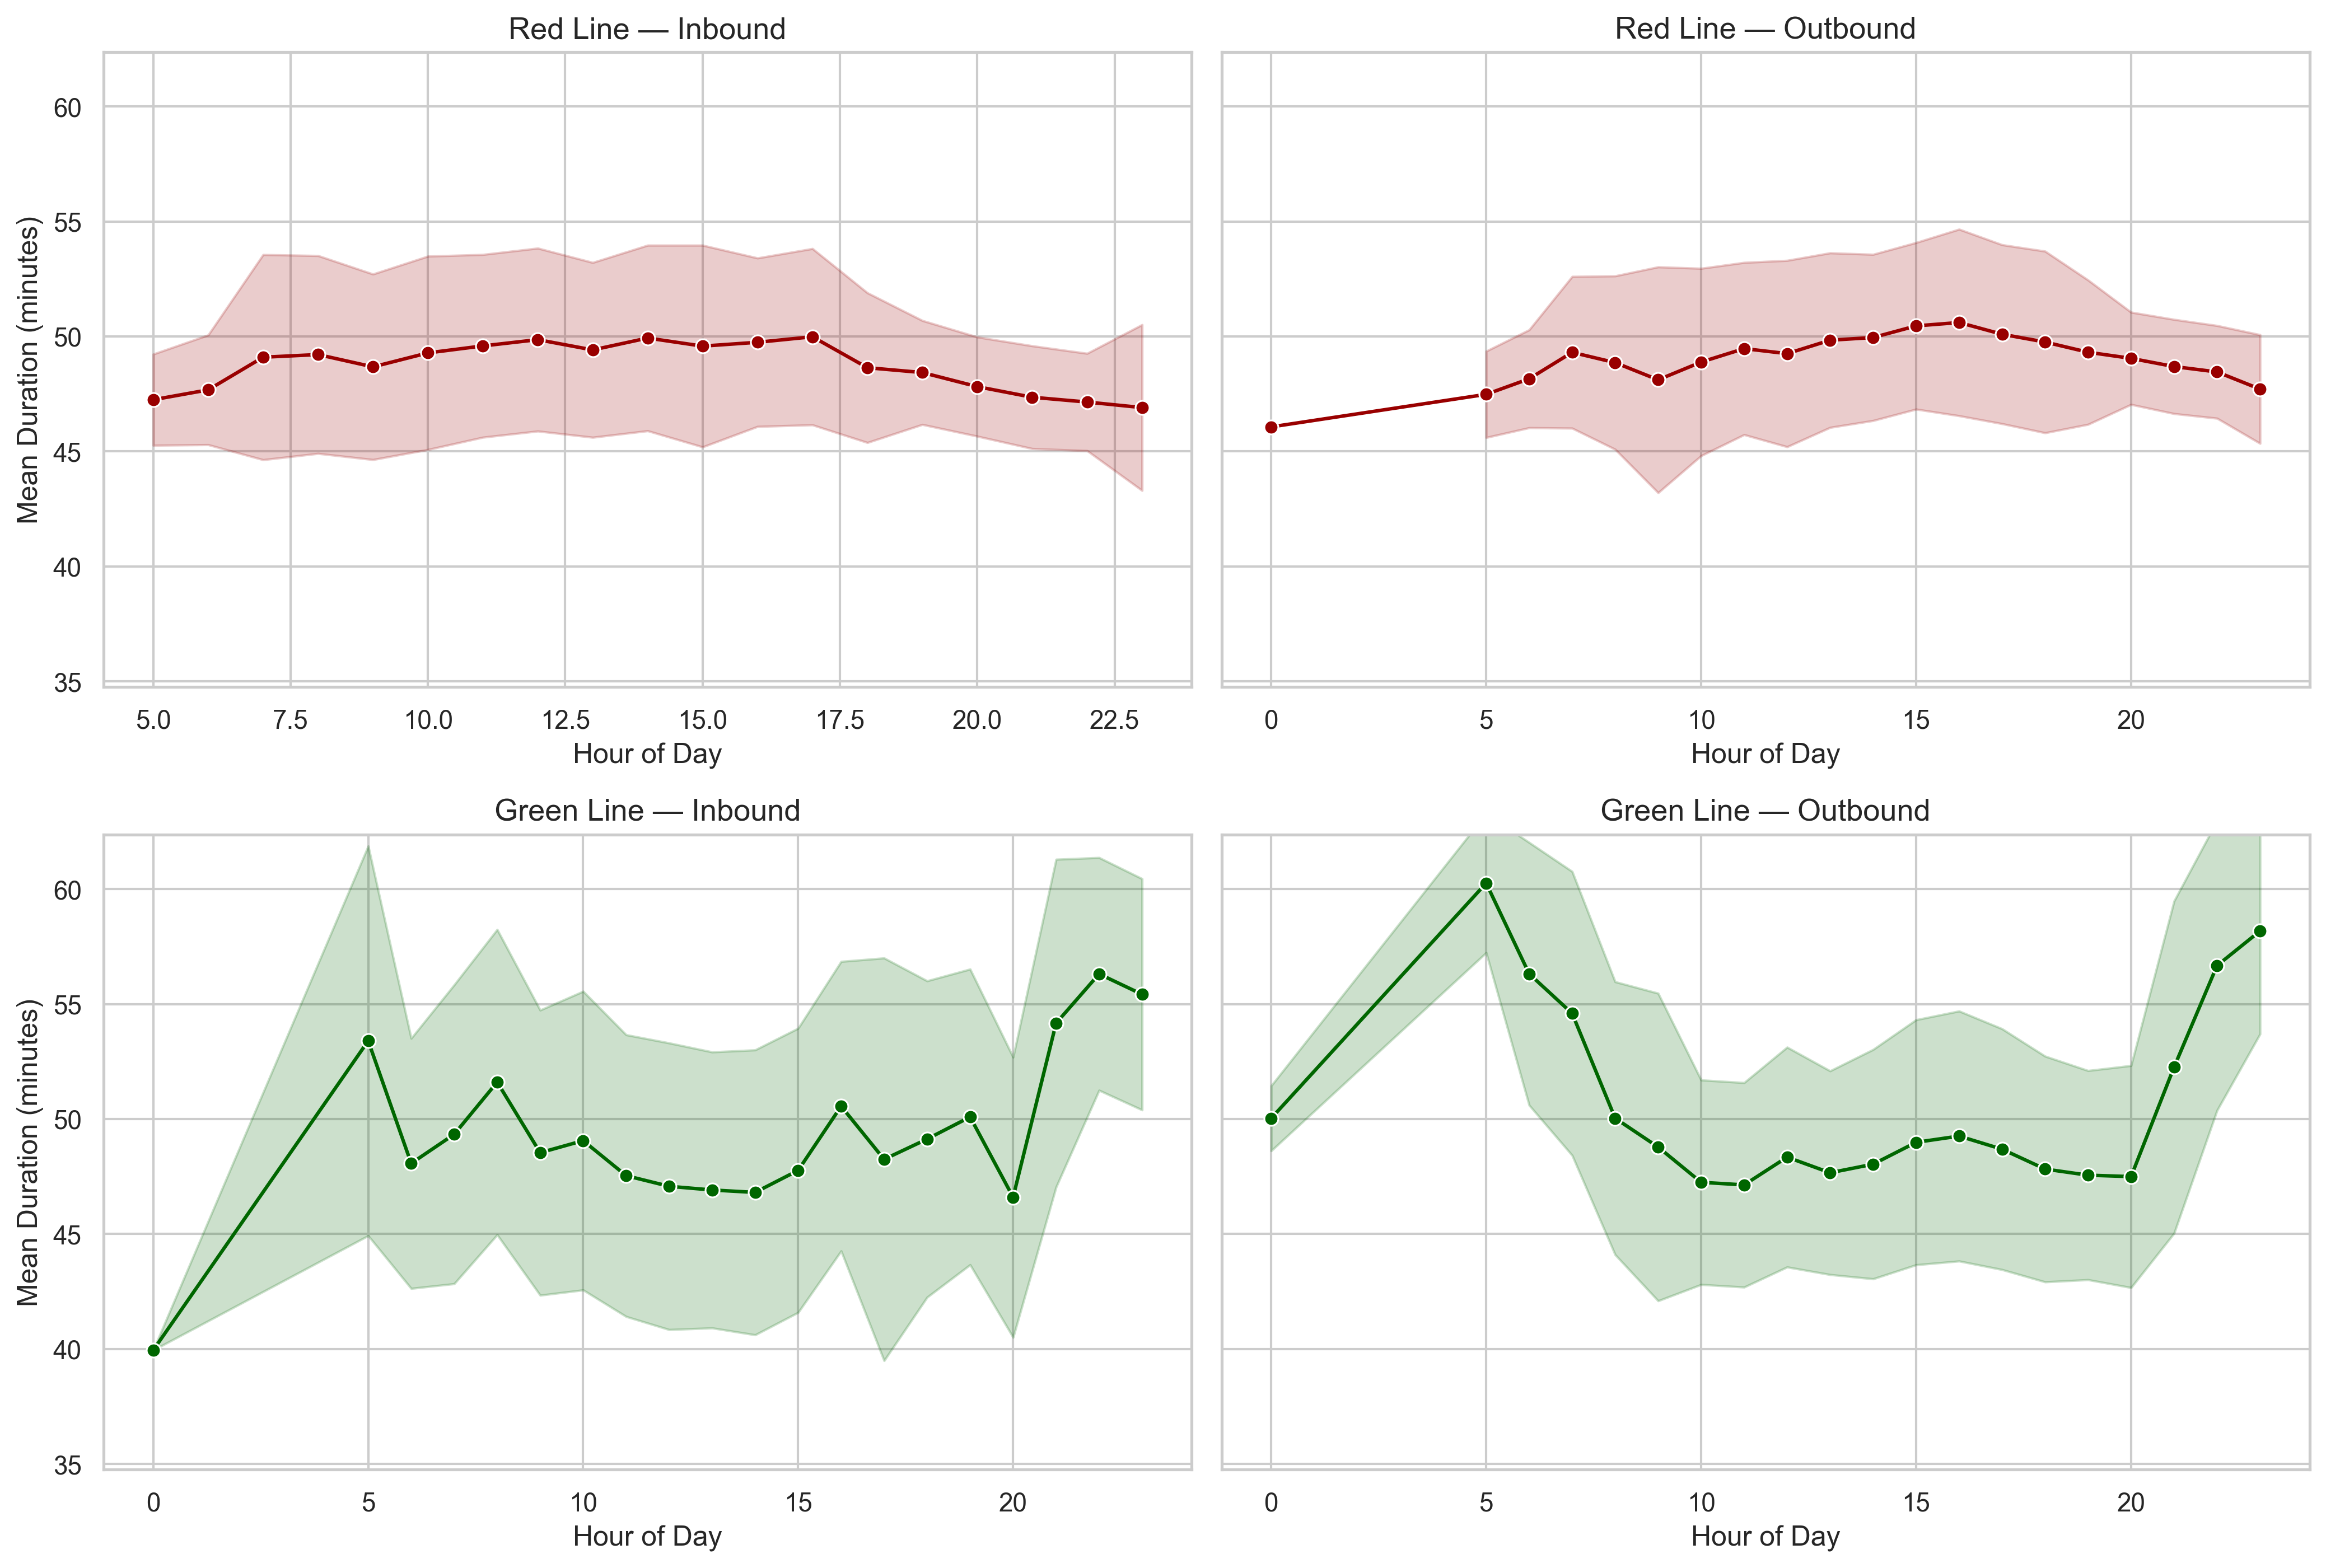
\includegraphics[width=\textwidth]{figures/appendix_figures/journey_duration/duration_hourly_combined_recovery.png}
    \caption*{By Hour}
  \end{subfigure}
  \hfill
  \begin{subfigure}[t]{0.49\textwidth}
    \centering
    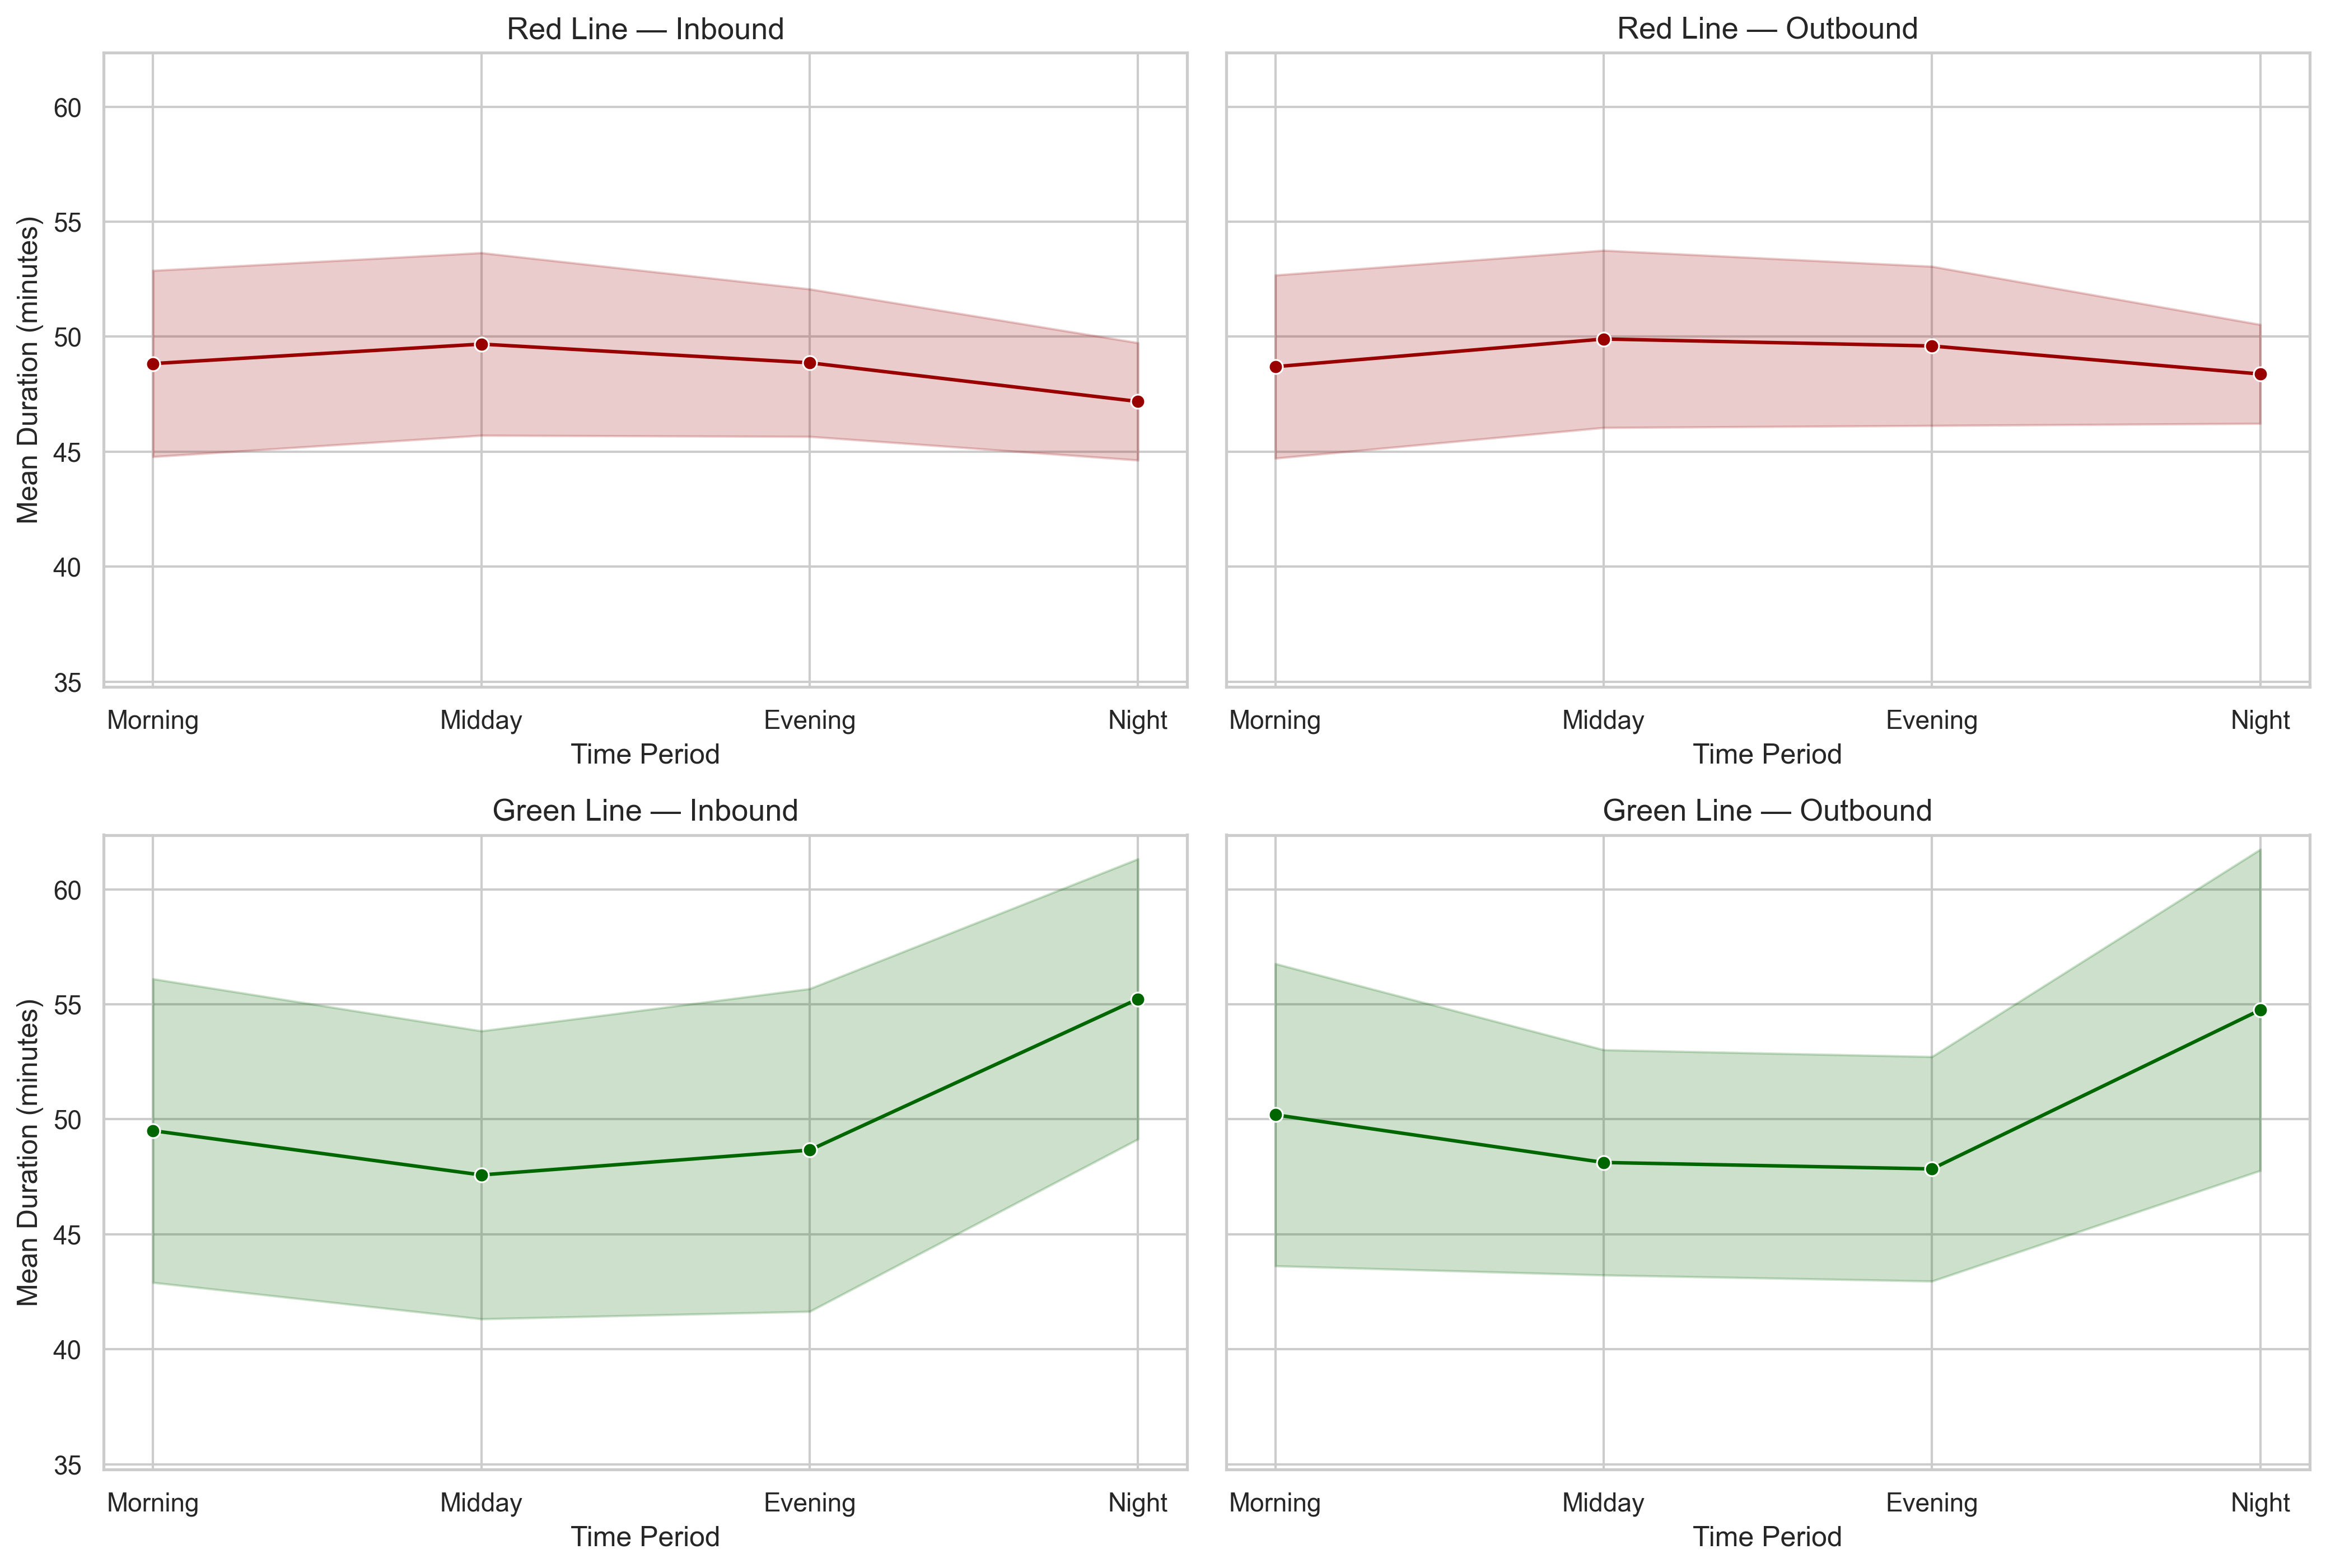
\includegraphics[width=\textwidth]{figures/appendix_figures/journey_duration/duration_period_combined_recovery.png}
    \caption*{By Time-of-Day}
  \end{subfigure}
  \caption{Recovery}
\end{figure}

\begin{figure}[H]
  \centering
  \begin{subfigure}[t]{0.49\textwidth}
    \centering
    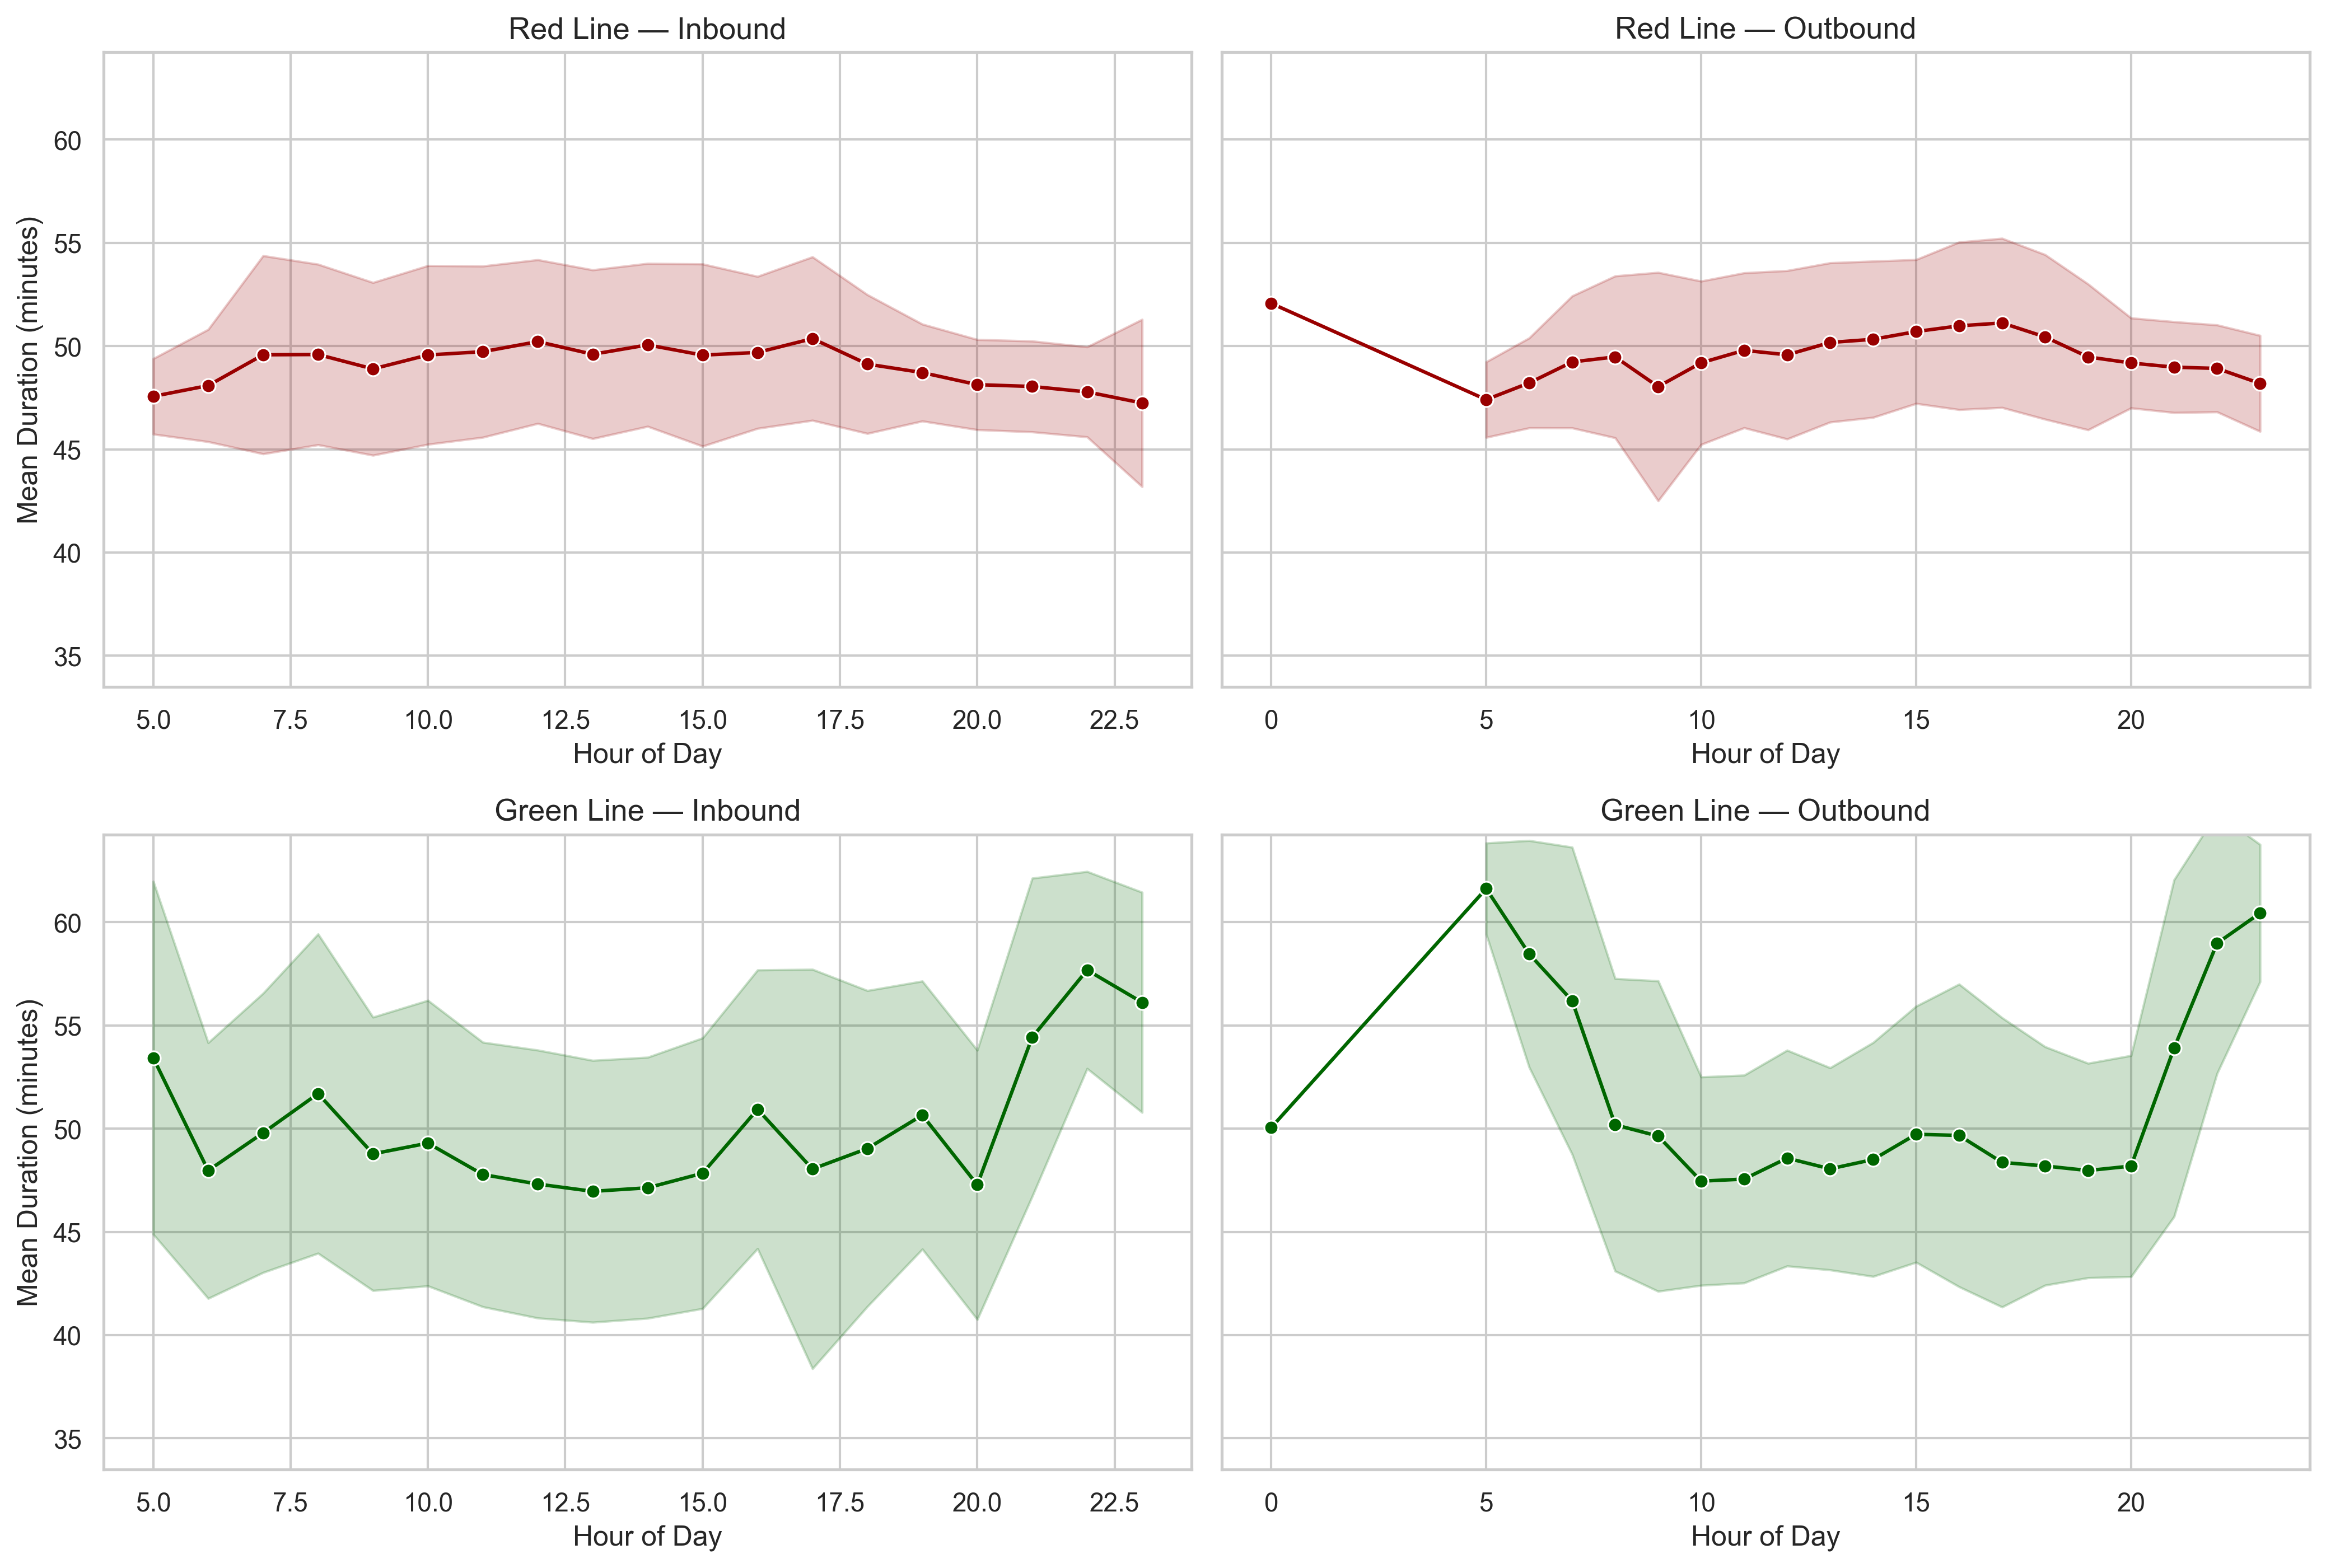
\includegraphics[width=\textwidth]{figures/appendix_figures/journey_duration/duration_hourly_combined_postcovid.png}
    \caption*{By Hour}
  \end{subfigure}
  \hfill
  \begin{subfigure}[t]{0.49\textwidth}
    \centering
    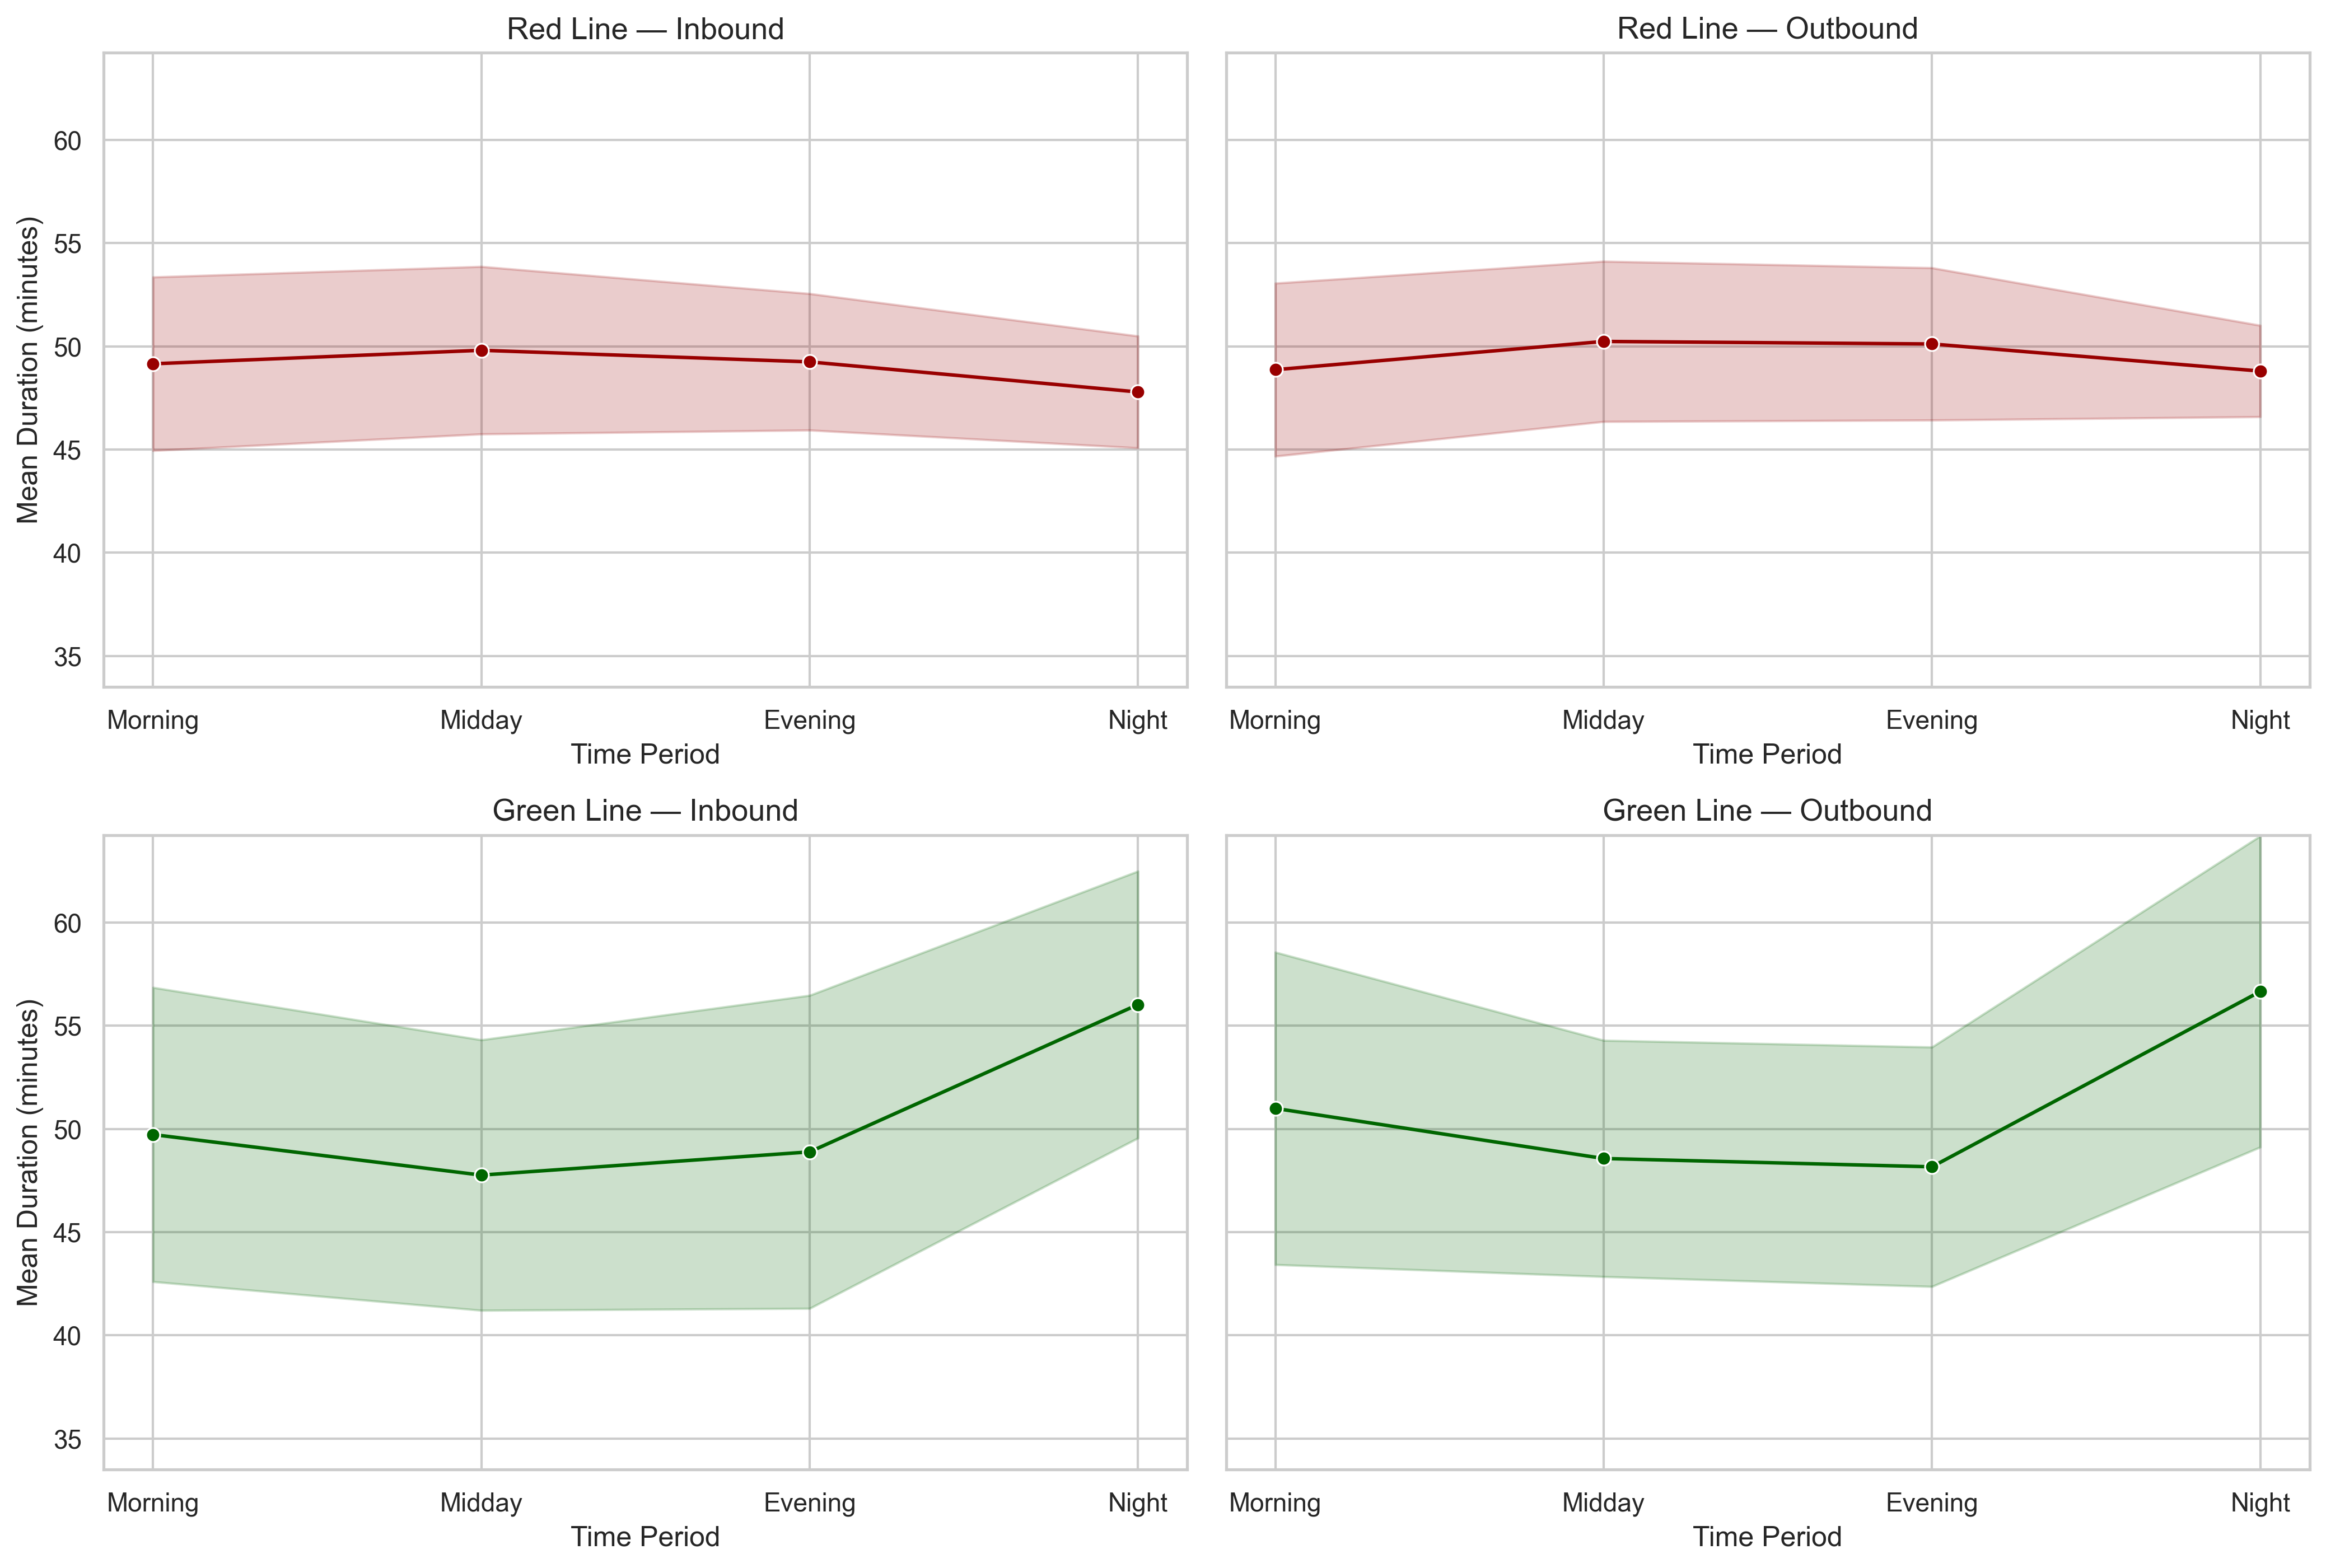
\includegraphics[width=\textwidth]{figures/appendix_figures/journey_duration/duration_period_combined_postcovid.png}
    \caption*{By Time-of-Day}
  \end{subfigure}
  \caption{Post-COVID}
\end{figure}
